% Terry Tao, on writing: https://terrytao.wordpress.com/advice-on-writing-papers/

% https://fenicsproject.org/olddocs/dolfin/1.5.0/python/demo/documented/stokes-iterative/python/documentation.html
%
%
%
%
%

% Preamble
% <<<
\documentclass[11pt,a4paper]{memoir}
\setsecnumdepth{subsection}
\setcounter{tocdepth}{2}
\setlrmarginsandblock{3cm}{3cm}{*} % Centre adjustment
\setulmarginsandblock{2.5cm}{*}{1}
\checkandfixthelayout 

\usepackage{amsmath}
\usepackage{amssymb}
\usepackage{mathtools}
\usepackage{microtype}
\usepackage{dirtytalk}
\usepackage{relsize}
\usepackage{csquotes}
\usepackage{epigraph}
\usepackage{physics}
\usepackage{cancel}
\usepackage{bm}
\usepackage{float}
\usepackage{algorithm2e}
% \RestyleAlgo{ruled}
\usepackage{subfig}
\usepackage{stackengine}
\usepackage[bookmarks]{hyperref}

\newcommand{\bb}{\begin{bmatrix}}
\newcommand{\bbe}{\end{bmatrix}}
\newcommand{\pr}{{\prime}}
\newcommand{\ppr}{{\prime\prime}}
\newcommand{\pppr}{{\prime\prime\prime}}
\newcommand{\inner}[1]{\left<#1\right>}
\newcommand{\fancyA}{\mathcal{A}}
\newcommand{\fancyL}{\mathcal{L}}
\newcommand{\fancyN}{\mathcal{N}}
\newcommand{\fancyP}{\mathcal{P}}
% \newcommand{\norm}[1]{\left\Vert#1\right\Vert}
\newcommand{\om}{{\Omega}}
\newcommand{\pom}{{\partial\Omega}}
\newcommand{\omn}{{\Omega_0}}
\newcommand{\pomn}{{\partial\Omega_0}}
\newcommand{\diver}{\text{div}}
\newcommand{\Part}[2]{\frac{\partial #1}{\partial #2}}
% footnotes
\renewcommand\footnoterule{}

\newcommand{\todo}[1]{\vskip 0.1in \hrule \vskip 0.03in {#1} \vskip 0.03in \hrule \vskip 0.1in}
% >>>

\begin{document}
\title{\Huge \textbf{The finite element method for the Navier-Stokes equations}}
\author{Lucas Payne}

\maketitle

\tableofcontents

\chapter{Mechanics}

\chapterprecishere{
Corpus omne perseverare in statu suo quiescendi vel movendi uniformiter in directum, nisi quatenus a viribus impressis cogitur statum suum mutare.
\\\\
Mutationem motus proportionalem esse vi motrici impressae, \& fieri secundum lineam rectam qua vis illa imprimitur.
\\\\
Actioni contrariam semper \& aequalem esse reactionem: sive corporum duorum actiones in se mutuo semper esse aequales \& in partes contrarias dirigi.
\par\raggedleft \textup{Newton \cite{newton}}}
% \section{Newton's laws of motion} % <<<
% 
% Newton's three laws, namely those of inertia, force, and equilibrium, have found universal success in application
% to mechanical systems such as the pendulum, the motion of a rigid body, the evolution of a bending beam, and, as we shall see,
% the motion of a fluid. \textit{Mechanics} could be thought of as the study of physical motion, but the word ``physical'' might be misleading.
% Newton's principles are mathematical in nature, applicable to the study of motion in a general sense as some unambiguously
% measurable state which evolves in time.
% 
% \subsection{Symmetry, momenta, and inertia}
% Mechanics as a theory of physical motion will require a definition of physical motion. A first attempt might be to posit
% that ``physical states'' are representable as points in a finite-dimensional manifold, which we call the configuration space $C$, which is the case for typical
% notions of state such as the two angles in a double pendulum, or the position and orientation of a rigid body. We might define a motion as
% a continuous time-parameterised curve
%     $$\gamma: [t_1, t_2] \rightarrow C.$$
% 
% % (--- motivation of $F = ma$, and momenta as fundamental quantity).
% 
% We start in the middle:
% \begin{equation}
%     \text{Total force = change of momentum}.
% \end{equation}
% In this form, Newton's second law of motion states that a (non-explanatory) measurement of change of momentum will be called ``force''.
% 
% 
% 
% % >>>
% \section{The Euler-Lagrange equations: \small{From $F = ma$ to $\Part{\fancyL}{q} - \frac{d}{dt}\Part{\fancyL}{\dot{q}} = 0$}} % <<<
% \subsection{A Lagrangian of a mechanical system}
% Force is an intensive measurement of the change in momentum. In the language of calculus,
% \begin{equation}\label{force_equation}
%     \int_{s_1}^{s_2} F\,dt = \fancyP(s_2) - \fancyP(s_1)
% \end{equation}
% for all time subintervals $[s_1, s_2] \subset [t_1, t_2]$. If we restrict $F$ to be conservative and a function only of position $q$, then we may
% let $F = -\Part{V}{q}$ for some potential function $V$. Suppose also that $\mathcal{P} = \Part{T}{\dot{q}}$ for some potential function
% (called the ``kinetic energy'') independent
% of position $q$. We then define a Lagrangian of the mechanical system to be
%     $$\fancyL(q, \dot{q}, t) = T(\dot{q}, t) - V(q, t) = \text{kinetic} - \text{potential}.$$
% By definition, we have the force equation \eqref{force_equation} as
%     $$-\int_{s_1}^{s_2} \Part{\fancyL}{q}\,dt = \Part{\fancyL}{\dot{q}}(s_2) - \Part{\fancyL}{\dot{q}}(s_1).$$
% The step toward the calculus of variations (---)
% \begin{equation}\label{el_inner_product_sum}
%         \int_{s_1}^{s_2} \Part{\fancyL}{q}h\,dt + \int_{s_1}^{s_2} \Part{\fancyL}{\dot{q}}\frac{dh}{dt}\,dt = 0
%     \quad\equiv\quad    \left<\Part{\fancyL}{q}, h\right> + \left<\Part{\fancyL}{\dot{q}}, \frac{dh}{dt}\right> = 0.
% \end{equation}
% Adjointness of differential operator $\frac{d}{dt}$ to $-\frac{d}{dt}$, and integration by parts. (---)
% By linearity, we then get the reformulation of \eqref{el_inner_product_sum} as
% \newcommand{\gateauxlagrangian}{\Part{\fancyL}{q} - \frac{d}{dt}\Part{\fancyL}{\dot{q}}}
%     $$\left<\gateauxlagrangian, h\right> = 0$$
% for all perturbation functions $h$.
% 
% \subsection{The first variation of a functional}
% In the calculus of variations, $\gateauxlagrangian$ is an instance of the \textit{G\^ateaux derivative}, also called the ``first variation'' of
% the functional
% \begin{align*}
%     S[q] \coloneqq \int_{t_1}^{t_2} \fancyL(q, \dot{q}, t)\,dt.
% \end{align*}
% The first variation measures response of the value of $S$, called the \textit{action}, to perturbations of the (differentiable) input function $q$,
% and is denoted
% \begin{equation}
%     \frac{\delta S}{\delta q(t)} \coloneqq \gateauxlagrangian.
% \end{equation}
% The first variation is linear in the perturbation function, and so another term for the G\^ateaux derivative could be ``functional gradient''.
% Setting this to zero gives the Euler-Lagrange equations, and the practice of determining trajectories of motions as stationary curves of the action is called the ``principle of stationary action''.
% 
% \subsection{From the Lagrangian to the equations of motion}
% In the framework of Lagrangian mechanics, $\fancyP \coloneqq \Part{\fancyL}{\dot{q}}$ is the momentum. If there are $d$ degrees of freedom
% in the mechanical system, and we suppose that $q_1,\cdots,q_d$ are (local) variables of state, then we say that $\fancyP_i \coloneqq \Part{\fancyL}{\dot{q}_i}$
% are \textit{conjugate} to the $q_i$.
% 
% (---) By inducing the equations of motion by a Lagrangian, we get systems with a ``physical interpretation'' with ``physically meaningful'' force measurements.
% 
% \subsection{Why ---?}
% These variational ideas appear because, no matter if our configuration space is finite-dimensional, time forms a continuum, and therefore if we
% globally consider the calculus of the motion as a whole, it must be a ``variational'' calculus. (---)
% 
% (---) Physical process, conservation laws, conservative forces (hint at thermodynamics limiting the range of stress tensors?)
% 
% When we consider mechanical models of continuum processes, we will see that these same ideas appear in the spatial dimensions too.
% A variational understanding of a continuum mechanics model leads very easily to a class of methods called Galerkin methods for solving
% the corresponding (PDE) equations of motion.
% 
% 
% % >>>

The calculus of variations.


\chapter{Continuum mechanics}
% Continuum Mechanics

\section{Introduction}
 % <<<
--- Introduction.

Although the focus later will be on fluid mechanics, a large set of fundamental concepts of solid and fluid mechanics
are the same. The key distinction appears when one focuses on displacements and materials with ``shear strength'' (solids)  versus flows
and materials with no shear strength (common fluids).

% >>>

\section{Transport}
% <<<
% Introduction
% <<<
Before considering continuum processes in the framework of Newtonian and Lagrangian mechanics, we will look at a fundamental notion of a ``motion''
of a point in a function space. Many continuum models in physics, such as the heat equation,
Maxwell's equations, and the equations of fluid motion, are formed by \textit{conservation equations}. These laws posit that the
evolution of the state (represented by a function) is
due to the transport of the quantity that the function measures, which is either pushed around (by some flux either predetermined or dependent on the current state),
introduced into the system at sources, or leaves the system at sinks.

% (figure of some manifold embedded in space, and some vector field pushing quantity around)
\begin{center}
\includegraphics[angle=90,page=11,width=0.56\linewidth]{figures/2.pdf}
\end{center}

We consider here the transport of quantities (scalar, vector, and tensor) on a general finite-dimensional manifold $M$,
colloquially called ``the continuum''. All transporting vector fields (or flux functions) are considered to be tangent to this manifold $M$.
% >>>
\subsection{Continuity equations and conservation laws}\label{conservation_laws}
% <<<
\subsubsection{The integral form of a continuity equation}
Consider some spatial quantity $\phi$ on $M$ and a flux function $j$ which by which
this quantity flows around $M$. For clarity, we will begin by specializing $\phi$ to be a scalar, although later we will find it useful to
transport vector quantities such as momentum. By definition we want this flux function to just push quantity around.
The entering and exiting of quantity into and out of the system is determined by some arbitrary source function $s$ (of the same kind as $\phi$). These variables are related by the
conservation condition
\begin{equation}\label{continuity_equation}
    \frac{d}{dt} \int_{\Omega_0} \phi\,dx = \int_{\Omega_0} s\,dx + \int_{\pomn} \phi j \cdot \left(-\hat{n}\right)\,dx
\end{equation}
for arbitrary control volumes $\Omega_0$ in the continuum. The term $-\hat{n}$ denotes the inward-pointing normal to the boundary of the control volume. This simply says that the change in the total quantity in the fixed control volume is accounted for exactly by that quantity pushed through the boundary by the flux function $j$, and the internal sources and sinks of quantity $s$.
% --- $s_B$ as a boundary term? Why introduce this? Seems to be needed for the derivation of surface forces.
% (--- It may be useful to add $s_G$ as a boundary source term at $\pomn \cap \pom$ so Dirac delta ideas don't need to be used for non-fluxed boundary source (or, for example, the domain might be a subdomain where the transported function is unknown outside, so the term is introduced through $s_G$.))

\subsubsection{The differential form of a continuity equation}
A common technique in continuum modelling is the use of Stokes' theorem to simplify integral expressions.
Stokes' theorem and its specialisations (such as the divergence theorem and Green's theorem) are really \textit{definitions} of pointwise quantities
such as the divergence and curl as limits of these integral expressions for arbitrarily small regions.

\begin{equation}
    \nabla\cdot v \coloneqq \lim_{\epsilon \rightarrow 0} \frac{1}{\pom_\epsilon}\int_{\pom_\epsilon}v\cdot\hat{n}\,dx.
\end{equation}
\begin{equation}
    \int_{\pom}v\cdot \hat{n}\,dx = \sum_{i\in\mathcal{I}}\int_{\pom_i}v\cdot \hat{n}\,dx.
\end{equation}
\begin{equation}
    \int_{\pom}v\cdot \hat{n}\,dx = \int_\om \left[\lim_{\epsilon \rightarrow 0}\frac{1}{\pom_{x,\epsilon}}\int_{\pom_{x,\epsilon}}v\cdot\hat{n}\,dx^\prime\right]\,dx.
\end{equation}


Equation \eqref{continuity_equation} becomes
\begin{equation}\label{continuity_equation_differential}
    \Part{\phi}{t} = s - \nabla\cdot (\phi j)
\end{equation}
assuming that $\phi j$ is sufficiently differentiable such that the limiting integral exists.
Continuity relations are most naturally expressed in form \eqref{continuity_equation}, while the form
\eqref{continuity_equation_differential} may be more useful for techniques such as finite differences.
Later, when we discuss numerical methods for solving continuum models, we will not take this route. The methods of interest, \textit{Galerkin} methods,
work naturally with the integral form \eqref{continuity_equation}.
It will be seen later that some constructions in the presentation of Galerkin methods, such as the ``weak form'' of a PDE, simply undo the differentialisation
(for example \eqref{continuity_equation_differential}) of the original integral form of physical PDEs (for example \eqref{continuity_equation}).
% (--- note: Maybe not exactly, as the integral conservation is quantified over regions, while the weak form is quantified over test functions,
% which still need to be sufficiently differentiabile. But I think that this must express the same continuity relation.)
% >>>
\subsection{The Reynolds transport theorem}
% <<<
\subsubsection{The integral form of Reynolds transport}
With our integral formulation of a continuity relation \eqref{continuity_equation}, the control volume $\Omega_0$ is fixed.
We may change our perspective by considering, in addition to the flux function $j$ (which transports quantity $\phi$), another
vector field $\hat{u}$ which will transport our control volume $\Omega_0$. The rate of change of some time-dependent quantity $\gamma$ in this
\textit{moving} control volume is expressed as
\begin{equation}\label{reynolds_rate_of_change}
    \frac{d}{dt}\int_{\Omega_0(t)}\gamma\,dx,
\end{equation}
where $\Omega_0(t)$ implicitly denotes that $\Omega_0$ is being transported under the flow of $\hat{u}$.
Clearly, this rate of change of quantity $\gamma$ is due to the motion of the control volume,

% \vskip 0.2in
% (a picture of positive and negative contributions at the boundary)
% \vskip 0.2in
\begin{center}
\includegraphics[angle=90,page=7,width=0.66\linewidth]{figures/2.pdf}
\end{center}

as well as internal changes of $\gamma$ inside the (fixed) control volume.
The formal expression of these contributions to the rate of change \eqref{reynolds_rate_of_change} is
\begin{equation}\label{reynolds_transport_theorem}
    \frac{d}{dt}\int_{\Omega_0(t)}\gamma\,dx = 
        \int_{\Omega_0(t)}\Part{\gamma}{t}\,dx + \int_{\partial\Omega_0(t)}\gamma \hat{u}\cdot\hat{n} \,dx.
\end{equation}
This result is called the \textit{Reynolds transport theorem},
a generalisation of Feynman's popularised ``differentiation under the integral sign'' \cite{feynman_trick},
otherwise named the Leibniz integral rule. See, for example, \cite{leal} for a formal derivation of \eqref{reynolds_transport_theorem}.
\subsubsection{The differential form of Reynolds transport}
 In the limit, with the routine application of Stokes' theorem, we can differentialise \eqref{reynolds_transport_theorem}
to get
\begin{equation}\label{reynolds_transport_theorem_differential}
    % \frac{d_{\hat{u}}\gamma}{d_{\hat{u}}t} = \Part{\gamma}{t} + \nabla \cdot(\gamma \hat{u}),
    \frac{d}{dt}\int_{\Omega_0(t)}\gamma\,dx \quad\longrightarrow\quad \Part{\gamma}{t} + \nabla \cdot(\gamma \hat{u}),
\end{equation}
as $\Omega_0$ becomes small.
The right-hand-side of \eqref{reynolds_transport_theorem_differential} measures
the change in volume of a quantity when a small control volume around the point of evaluation is moved, expanded or contracted by the flow field $\hat{u}$.

\subsubsection{Reynolds transport applied to a continuity equation}
Letting our quantity $\gamma$ in \eqref{reynolds_transport_theorem} be the quantity $\phi$ transported by flux function $j$,
described in continuity equation \eqref{continuity_equation}, we get a specialised form of the Reynolds transport theorem for continuity equations.
Term $\Part{\gamma}{t}$ in \eqref{reynolds_transport_theorem} becomes $\Part{\phi}{t}$ in the differential form of the continuity equation \eqref{continuity_equation_differential}, giving
\begin{equation}\label{reynolds_transport_continuity_equation}
\begin{split}
    \frac{d}{dt}\int_{\Omega_0(t)}\phi\,dx
        &= \int_{\Omega_0(t)}-\nabla\cdot(\phi j) + s\,dx + \int_{\partial\Omega_0(t)}\phi \hat{u}\cdot\hat{n} \,dx \\
        &= \int_{\Omega_0(t)}s\,dx + \int_{\partial\Omega_0(t)}\phi (\hat{u} - j)\cdot\hat{n} \,dx
\end{split}
\end{equation}
by Stokes' theorem. This has a clear interpretation.
The $\hat{u} - j$ term is due to us wanting to measure the contributions to the total $\phi$ due to the moving boundary of
$\Omega_0$, where the motion that matters is \textit{relative} to the flux of the quantity $j$. Specifically, if we move the control volume by
the same flux function $j$ (letting $\hat{u} = j$), we get
\begin{equation}\label{lagrangian_transport}
    \frac{d}{dt}\int_{\Omega_0(t)}\phi\,dx
        = \int_{\Omega_0(0)}s\,dx.
\end{equation}
In fact, \eqref{lagrangian_transport} is just another form for the conservation law \eqref{continuity_equation},
where the ``frame of reference'' for measurement of $\phi$ follows the transport of $\phi$. This simply means that as we follow some volume of quantity
original situated in $\Omega_0$, a conservation law posits that the only change detected is due to the source function $s$. In differential form
\eqref{lagrangian_transport} becomes
\begin{equation}\label{lagrangian_transport_differential}
    \Part{\gamma}{t} + \nabla \cdot(\gamma \hat{u}) = s,
\end{equation}
a succint equivalent to \eqref{continuity_equation_differential}.
The idea of following the flow while making measurements is called the \textit{Lagrangian} perspective, in contrast to the \textit{Eulerian}, fixed, perspective.
% >>>
\subsection{Incompressible and compressible transport}
% <<<
% While the continuity equation \eqref{continuity_equation} gives us a general conservation law, transporting some quantity
% through our continuum (---without loss of generality, assume some domain $U \subset \mathbb{R}^2$), this is simply analogous
% to how general vector fields on the configuration space describe the evolution of a state in a finite-dimensional mechanical system
% (--- note that the ``vector field'' in consideration for the continuum case is really a ``vector field of vector fields'' on $C$, since
% a vector in the tangent space of $C$ here would be the vector field giving transport.
% Need to clearly distinguish these notions and use clear terminology, as it could be confusing).
Analogous to constraints on the motion of a finite mechanical system,
% (--- section on Lagrangian mechanics should have an example of constraints of motion for a pendulum)
we can constrain possible movement of our continuous quantity to \textit{incompressible transport}. Much like how, in the framework of Lagrangian mechanics,
constraints on motion are implicitly enforced by strong ``virtual forces'', constraining transport to be non-compressing will lead to
the notion of \textit{pressure}, derived in section \ref{pressure_derivation}.

\subsubsection{Incompressibility}
Incompressibility of control volumes gives a constraint on the form of a flux function $j$.
We call this constrained flux function $j$ non-compressing.
By incompressibility we mean that a control volume being transported by $j$ will have
constant volume. While $j$ may transport other quantities, we express incompressibility by requiring the flux function to transport a constant ``volume quantity''
with a corresponding null source function,
    $$\phi_{\text{vol}} = 1,\quad s_{\text{vol}} = 0.$$
The corresponding conservation law, in differential form \eqref{continuity_equation_differential}, is
\begin{equation}\label{volume_conservation_law}
    \Part{\phi_{\text{vol}}}{t} = -\nabla \cdot (\phi_{\text{vol}}j) + s_{\text{vol}}
        \quad\Rightarrow\quad \nabla\cdot j = 0.
\end{equation}
This is our non-compressing constraint on $j$, and has a clear interpretation, as there is a non-zero divergence of $j$ if and only if
there is an inward or outward flux which would contract or expand a transported control volume.
% >>>
\subsection{Transport of vector and tensor quantities}
% <<<
All previous discussion on the transport of scalar quantities applies trivially to vector and tensor quantities.
This will soonest be of use in the discussion of conservation of linear momentum, a vector quantity
% (---should this be mentioned? It doesn't fit into the
% framework so far as there is no notion of position map, this might be confusing and seem to imply ``linear momentum'' is natural for any continuum process).
However, some notational discussion is needed in order to establish differential forms of continuity equations and the Reynolds transport theorem.
\subsubsection{Reynolds transport of vector and tensor quantities}
For a general tensor quantity $\Gamma$, the integral form of Reynolds transport \eqref{reynolds_transport_theorem} is trivially
\begin{equation}\label{reynolds_transport_theorem_tensor}
    \frac{d}{dt}\int_{\Omega_0(t)}\Gamma\,dx
        \int_{\Omega_0(t)}\Part{\Gamma}{t}\,dx + \int_{\partial\Omega_0(t)}\Gamma \left(\hat{u}\cdot\hat{n}\right) \,dx.
\end{equation}
The step to the differential form \eqref{reynolds_transport_theorem_differential}, however, needs some thought
as rearranging
    $$\text{``}\Gamma\left(\hat{u}\cdot \hat{n}\right) = (\Gamma\hat{u})\cdot \hat{n}\text{''}$$
in order to apply the divergence theorem makes no sense. However, the divergence $\nabla \cdot$ was \textit{defined}
to evaluate the limit of this boundary integral for arbitrarily small $\Omega_0$. We therefore have a natural generalisation of the
divergence for arbitrary tensors $\Psi$, as the limit of the boundary integral of the \textit{contraction} of $\Psi$ with the outward normal
$\hat{n}$ (which is a contravariant vector). The divergence of a rank $n$ tensor is then a rank $n-1$ tensor,
\begin{equation}\label{tensor_divergence}
    \int_{\Omega_0} \nabla\cdot\Psi\,dx \coloneqq
        \int_{\partial{\Omega_0}} \Psi : \hat{n}\,dx.
\end{equation}
We can then rewrite $\Gamma \left(\hat{u}\cdot \hat{n}\right)$ in \eqref{reynolds_transport_theorem_tensor} as
    $$\Gamma \left(\hat{u}\cdot \hat{n}\right) = \left(\Gamma \otimes \hat{u}\right) : \hat{n},$$
where the tensor product $\otimes$ ``defers contraction'' of $\hat{u}$ with $\hat{n}$, by storing it as a component of product tensor $\Gamma \otimes \hat{u}$.
This leads to a differentialisation of \eqref{reynolds_transport_theorem_tensor},
\begin{equation}\label{reynolds_transport_theorem_tensor_differential}
    \frac{d_{\hat{u}}\Gamma}{d_{\hat{u}}t} = \Part{\Gamma}{t} + \nabla \cdot(\Gamma \otimes \hat{u}).
\end{equation}
% (--- interpretation of this. This does actually make sense from ``first principles'' rather than tensor algebra.)
\subsubsection{Conservation equations for vector and tensor quantities}
With the previous ideas from tensor algebra, it will be easy to describe continuity relations for transport of tensors. The integral form of the scalar continuity equation \eqref{continuity_equation}, generalised to transported tensor $\Phi$, trivially becomes
\begin{equation}\label{continuity_equation_tensor}
    \frac{d}{dt} \int_{\Omega_0} \Phi\,dx = \int_{\partial\Omega_0} \Phi \left(j\cdot (-\hat{n})\right)\,dx + \int_{\Omega_0} s\,dx.
\end{equation}
By the same tensor algebra as above we have
    $$
        \Phi \left(j\cdot (-\hat{n})\right) = -\left(\Phi \otimes j\right) : \hat{n},
    $$
giving \eqref{continuity_equation_tensor} in differential form as
\begin{equation}\label{continuity_equation_tensor_differential}
    \Part{\Phi}{t} = -\nabla\cdot (\Phi \otimes j) + s.
\end{equation}
% Finally, we may take a Lagrangian perspective on the transport of tensor $\Phi$ by letting the boundary transport in
% \eqref{reynolds_transport_theorem_tensor_differential}
% be the flux function, $\hat{u} = j$,
% and $\Gamma$ be the tensor $\Phi$ being transported by $j$, giving
% \begin{equation}\label{lagrangian_transport_tensor_differential}
%     \frac{d_j \Phi}{d_j t} = \cancel{-\nabla\cdot\left(\Phi\otimes j\right)} + s + \cancel{\nabla\cdot\left(\Phi\otimes j\right)} = s.
% \end{equation}
% (--- This shows that tensor transport is a trivial modification of the previous results.)
% \subsubsection{The meaning of tensor transport}
% --- show that this is just a trivial notational convenience, as e.g. vector transport can just be done component-wise.
% >>>
% >>>

\section{The kinematics of the continuum}
% <<<
% Introduction
% <<<
Transport equations are just one notion of ``physical motion'' in a continuum model.
These transport equations, with prescribed flux and source functions, determine a continuous process on a fixed
domain $M$. These conserved quantities are time-varying maps from $M$ to some measurement space of scalars or tensors.
Each map is a component of the total configuration space $C$, which clearly must be infinite-dimensional.
We now consider another component of $C$
which will let us model a physical domain with alterable shape.
In our discussion we will consider a fixed time interval $[t_1, t_2]$ in which our physical motions will take place.
% >>>
\subsection{Position maps}
% <<<
We may consider the manifold $M$ as the parametric domain of some points living in an ambient manifold $N$.
We will call this the ``position map''
    $$y:M\times [t_1, t_2] \rightarrow N.$$
In general, $y$ needs not be continuous, differentiable, or invertible.
These restrictions are only introduced in accord to the physical meaning of the position map. For example, models of small beam deflections
may require continuity, and invertibility to prevent self-intersections.

% \vskip 0.2in
% (figure of abstract square domain mapping to a bent beam, and a figure of a map from a reference configuration to itself.)
% \vskip 0.2in
\begin{center}
\includegraphics[angle=90,page=8,width=0.5\linewidth]{figures/2.pdf}
\end{center}


As an example, suppose we are modelling the heat distribution of a 2D beam supporting a point load which is also a heat source.
We could model the beam geometry as a smooth invertible map $y: [0,1]^2\rightarrow \mathbb{R}^2$,
letting $M = [0,1]^2$ and $N = \mathbb{R}^2$. The heat distribution on the beam could be represented
by a function $h : M \rightarrow \mathbb{R}$, and a heat flux function $j$ could be pulled back to $M$ from $N$.

% \vskip 0.2in
% (picture of this)
% \vskip 0.2in
\begin{center}
\includegraphics[angle=90,page=9,width=0.55\linewidth]{figures/2.pdf}
\end{center}

Although this model is so far hopelessly incomplete, we can see that position maps and transport equations are fundamental tools
used for modelling the \textit{geometry} of a problem.


% \subsubsection{Displacement maps}
% --- possibly discuss.
% --- M is a subdomain of N, define a map which gives a displacement vector, which might only really make sense in Euclidean space.
% 
% \subsection{The configuration space of a continuum model}
% In sections (ref) and (ref) we discussed the mechanics of a physical system which can be encoded as a point in a finite-dimensional configuration manifold
% $C$. Clearly, however, if we consider $x$ a part of the physical state, the space of states will be infinite-dimensional. $x$ is just one possibly
% useful state variable which we have used for demonstration. We may, for example, consider continuum models for advection-diffusion processes \cite{turing} on some non-moving domain, without the use of a position function. $x$ is an instance of a \textit{point valued} map, in constrast to quantity (scalar or tensor) valued maps
% discussed previously. (---discuss why continuity equations would not apply (?))
% 
% Continuum mechanics will study the physical motion of $x$, and other maps, where the equations of motion are, for example,
% transport equations. Each component of our state will have a corresponding velocity. In the case of the position map $x : M \times [t_1, t_2] \rightarrow N$,
% the velocity is a vector field which
% >>>
\subsection{Velocity}
% <<<
As in the mechanics of a particle, each component of our state $q \in C$ will have a corresponding velocity which ``generates'' a physical motion of that component.
In the case of the position map $y : M \times [t_1, t_2] \rightarrow N$, the velocity will be given by
a vector in the tangent space of $N$ at $y(x)$ for each parameter $x \in M$. This vector field is denoted $\dot{y}$.
This is the \textit{Lagrangian} description of motion. We will find it useful to instead use the \textit{Eulerian} description, where we measure the velocity of the position map in the position domain $N$. Formally we denote this Eulerian velocity by the letter $u$, ubiquitous in fluid mechanics, and let
    $$u(y, t) \coloneqq \dot{y}(y^{-1}(y, t), t)\quad \text{for all valid $y\in N$.}$$

\begin{center}
\includegraphics[angle=90,page=2,width=0.8\linewidth]{figures/2.pdf}
\end{center}

For some transported scalar quantity $\phi : M \times [t_1, t_2] \rightarrow \mathbb{R}$, the tangent space at each point of $\mathbb{R}$ is $\mathbb{R}$,
and therefore our velocity is represented by a scalar function $\Part{\phi}{t}$ giving local change in time of $\phi(x)$ for each $x \in M$.

% \vskip 0.2in
% (draw this)
% \vskip 0.2in
\begin{center}
\includegraphics[angle=90,page=3,width=0.8\linewidth]{figures/2.pdf}
\end{center}

We may denote our total velocities as a state variable $\dot{q}$. 
When we have state $q$, the corresponding velocity $\dot{q}$ will be in the tangent space of $C$ at $q$, denoted $T_q C$.
We can then define the space of velocities as the \textit{tangent bundle} of the configuration space,
    $$TC = \bigcup_{q \in C} T_q C.$$
% >>>
\subsection{The deformation and velocity gradients}\label{deformation_and_velocity_gradients}
% <<<
We may think of the mechanics of a particle as a special case of our continuum model, where
$M$ is a single point. In this case we have only one $x \in M$, so we cannot vary $x$.
However, for a continuum parameter domain $M$ we can take derivatives with respect to our parameter as well as time.
We can extract important geometric/kinematic information from the spatial derivatives of our position map $y$.

\subsubsection{The deformation gradient}
The gradient of the position map $y$ with respect to parameter $x \in M$ is called the \textit{deformation gradient}
\begin{equation}\label{deformation_gradient}
    \nabla y.
\end{equation}
The deformation gradient is equivalent to the \textit{Jacobian matrix}, used to compute the \textit{pushforward}
of tangent vectors under the displacement map.

% \vskip 0.2in
% (draw this)
% \vskip 0.2in
\begin{center}
\includegraphics[angle=90,page=4,width=0.5\linewidth]{figures/2.pdf}
\end{center}

The determinant of the Jacobian matrix is usually denoted $J = \det(\nabla y)$, and is called the Jacobian.

\subsubsection{The velocity gradient}
Letting $u$ be our Eulerian velocity as defined above, we may express the position map through an ODE,
\begin{equation}\label{position_map_ode}
\begin{split}
    \frac{d}{dt} y(x, t) = u(y(x, t), t),\quad
    y(x, 0) = y_0(x).
\end{split}
\end{equation}
It is common, especially in flow problems, to let $M$ be a subset of $N$ which is the ``initial geometry''.
In this case we could let the initial position map be the identity map
    $$y_0(x) = x \in M \subset N.$$
For example, given an initial disc in $\mathbb{R}^2$, we may prescribe a constant Eulerian velocity field $u$ and
see how the original disc is ``mixed''.

% \vskip 0.2in
% (draw this)
% \vskip 0.2in
\begin{center}
\includegraphics[angle=90,page=5,width=0.4\linewidth]{figures/2.pdf}
\end{center}


We can see that, in this case, it is meaningful to take spatial gradients in \eqref{position_map_ode} to derive an ODE for the deformation gradient $\nabla y$:
\begin{equation}\label{deformation_gradient_ode}
\begin{split}
    \nabla \left[\frac{d}{dt} y(x, t)\right] = \nabla u(y(x, t), t),\quad
    \nabla y(x, 0) = I,
\end{split}
\end{equation}
where $I$ is the identity tensor. This is easily visualised.

% \vskip 0.2in
% (draw this)
% \vskip 0.2in
\begin{center}
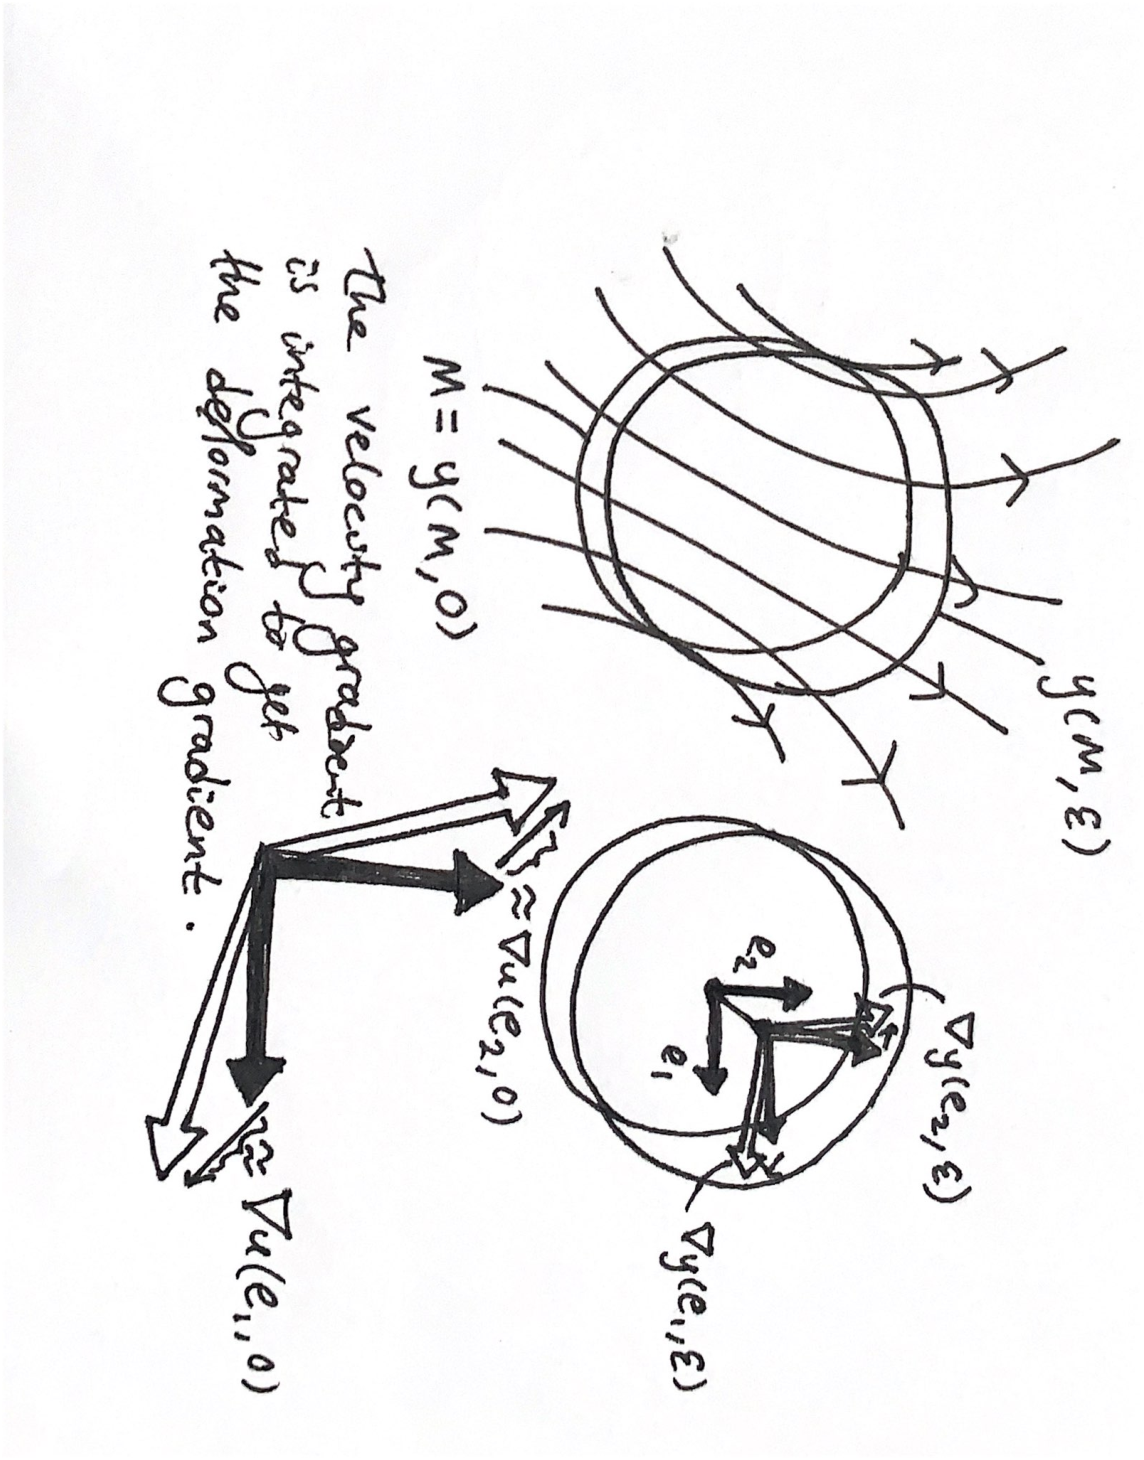
\includegraphics[angle=90,page=1,width=0.58\linewidth]{figures/1.pdf}
\end{center}

We can see that the term $\nabla u$ is a ``differential generator'' of the deformation gradient.
$\nabla u$ is called the \textit{velocity gradient}.

% Polar decomposition, symmetric and antisymmetric parts.
% >>>
\subsection{Material points and material derivatives}\label{material_points}
% <<<
\subsubsection{The material derivative}

Assuming an non-compressing flux function $u$ which transports quantity $\phi$, the differential form of the Reynolds transport theorem
\eqref{lagrangian_transport_differential} becomes
\begin{equation}
    \Part{\phi}{t} + \nabla\cdot(\phi u) = \Part{\phi}{t} + u\cdot\nabla\phi + \cancel{\phi \nabla\cdot u}.
\end{equation}
We define the \textit{material derivative} to be
\begin{equation}\label{material_derivative}
    \frac{D}{Dt} \coloneqq \Part{}{t} + u\cdot\nabla.
\end{equation}
It is a convention to leave the vector field $u$ implicit, as material derivatives are usually taken with respect to the velocity field.
This derivative \eqref{material_derivative} will turn out to measure ``per-volume'' quantities.

\subsubsection{Pieces of the continuum}
A \textit{material element} is a small piece of a continuum model which evolves with the displacement and flow.
In fluid dynamics this is also called a fluid parcel, although it should not be thought of as an object placed in the fluid, but
rather some tracer such as a non-diffusing dye.

% \vskip 0.2in
% (draw this)
% \vskip 0.2in
\begin{center}
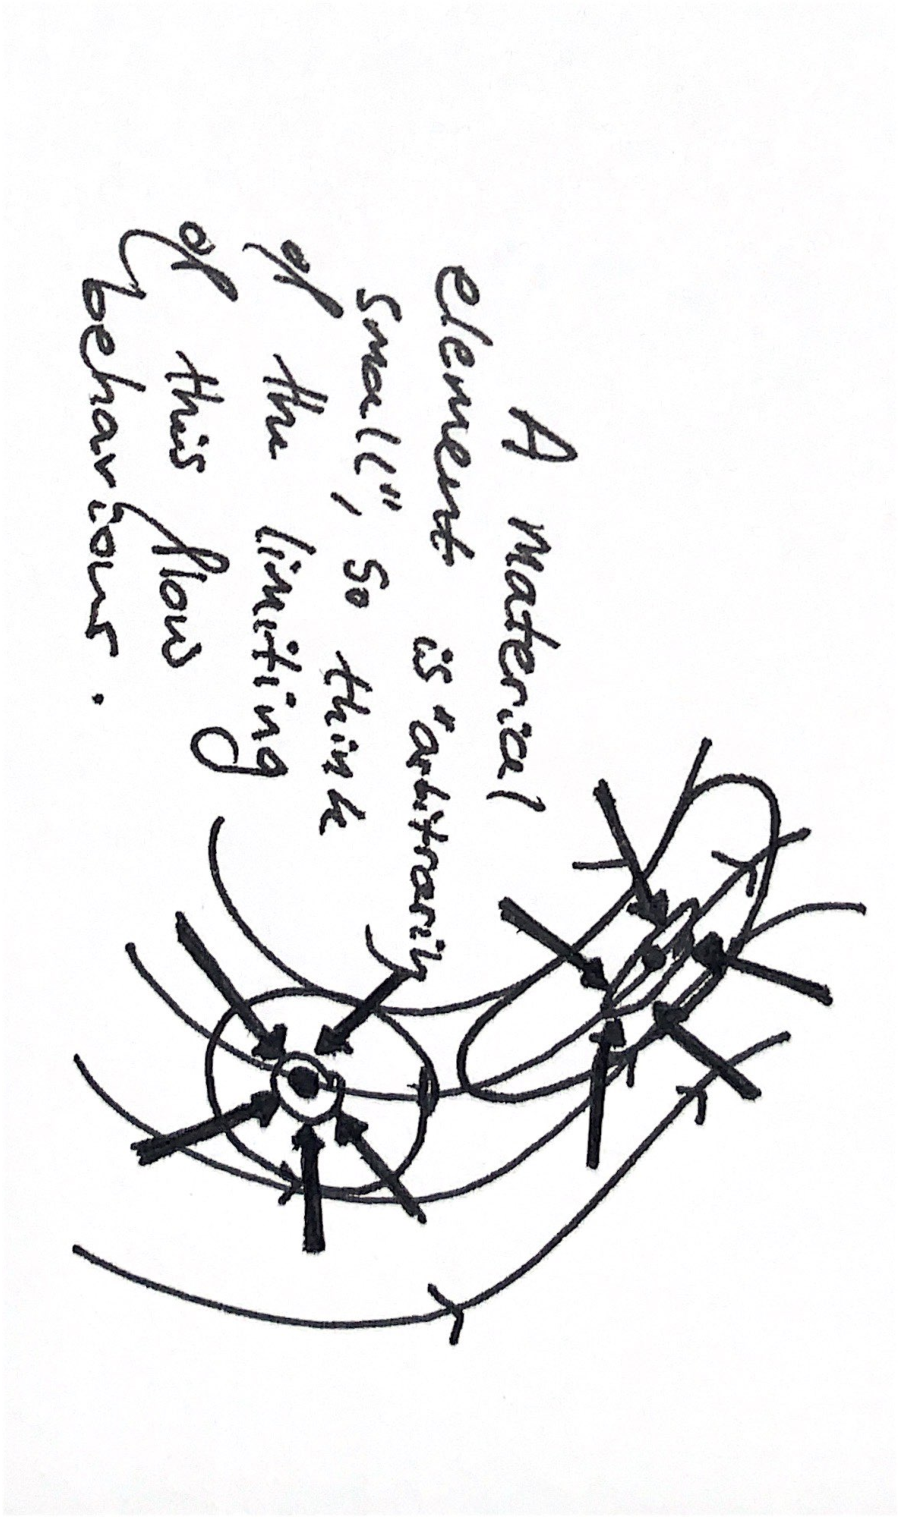
\includegraphics[angle=90,page=1,width=0.55\linewidth]{figures/2.pdf}
\end{center}

In continuum mechanics a \textit{material point} is the ideal point of the continuum, corresponding to some macroscopic averaging in physical models.
At a certain point, we can imagine an arbitrarily small fluid parcel being transported by the flow.
No matter how small this is, the parcel will still start to shear, expand, and contract due
to the flow.
The material derivative was defined as $\frac{D}{Dt} \coloneqq \Part{}{t} + u\cdot\nabla$. Notably this derivative contains no divergence term, and so does not
measure the
change of a quantity due to expansion and contraction of the arbitrarily small fluid parcel. Therefore we can think of the material derivative as acting
on \textit{per-volume} quantities.

% \vskip 0.2in
% (figure of a point mass flowing along a scalar field, and a mass with extent being compressed)
% \vskip 0.2in
\begin{center}
\includegraphics[page=2,width=0.66\linewidth]{figures/3.pdf}
\end{center}

% >>>
% >>>

\section{The dynamics of the continuum}
% <<<
\subsection{Conservation of mass}
% <<<
We will take for granted that there is some initial mass density function $\rho_0:M\rightarrow \mathbb{R}^+$
which we would like to conserve.
\subsubsection{The Lagrangian form of mass conservation}
As the position map $y$ evolves, for example under the action of Eulerian velocity field $u$ in the ODE \eqref{position_map_ode},
we would like a mass density function $\rho : N \rightarrow \mathbb{R}^+$ to be greater if the position map ``compresses'' the material,
and smaller if it ``stretches'' the material. Our aim is that the total mass measured in a control volume of $N$ is the same as in its initial configuration.
We can express this by the integral equation
\begin{equation}\label{lagrangian_mass_conservation}
    \int_{\omn} \rho_0(x)\,dx = \int_{y(\omn, t)} \rho(y, t)\,dy,
\end{equation}
where $y(\omn, t)$ denotes the domain pushed forward by the position map. By the usual change of variables formula we have
\begin{equation}\label{lagrangian_mass_conservation_cov}
    \int_{\omn} \rho_0(x)\,dx = \int_{\omn} \det(\nabla y)\rho(y(x,t), t)\,dx,
\end{equation}
where $J = \det(\nabla y)$ is the Jacobian, measuring the local change in the volume element due to the change of variables.

\vskip 0.2in
(draw this)
\vskip 0.2in

As \eqref{lagrangian_mass_conservation_cov} must hold identically for all $\Omega_0$, we have the localised conservation law
\begin{equation}\label{lagrangian_mass_conservation_local}
    \rho_0 = \det(\nabla y)\rho.
\end{equation}

\subsubsection{The Eulerian form of mass conservation}
Conservation law \eqref{lagrangian_mass_conservation_local} is simple. However, it is given in terms of absolute deformation gradient $\nabla y$.
Instead of asking how mass is distributed
in comparison to its initial configuration, we can ask how mass is transported by $u$.
This gives an instance of the continuity equation \eqref{continuity_equation}, where we have no source:
\begin{equation}\label{eulerian_mass_conservation}
    \frac{d}{dt} \int_{\omn} \rho \,dx + \int_{\pomn} \rho u\cdot \hat{n}\,dx = 0.
\end{equation}
With application of Stokes' theorem we have
\begin{equation}\label{eulerian_mass_conservation_local}
    \Part{\rho}{t} + \nabla \cdot (\rho u) = 0.
\end{equation}
Following \cite{leal}, there is a more geometrical statement of this equation, which will be useful when
we discuss ``material points''
By a divergence product rule \eqref{eulerian_mass_conservation_local} is equivalent to
\begin{equation}\label{eulerian_mass_conservation_local_material}
    \Part{\rho}{t} + u\cdot\nabla\rho + \rho\nabla\cdot u = 0
    \quad\Rightarrow\quad \frac{D\rho}{Dt} = -\rho\nabla\cdot u,
\end{equation}
where $\frac{D}{Dt}$ is the material derivative as defined in \eqref{material_derivative}.

% >>>
\subsection{Conservation of linear momentum}
% <<<
If we conserve the linear momentum $\rho u$, a ``quantity of motion'', under the flow of $u$, then we get a continuity equation
\begin{equation}\label{cauchy_continuity_traction}
    \frac{d}{dt}\int_{\Omega_0(t)}\rho u\,dx = \int_{\omn(t)} \rho g\,dx + \int_{\pomn(t)}\hat{t}\,dx,
\end{equation}
a specific realisation of the Lagrangian continuity equation \eqref{lagrangian_transport}. The Lagrangian perspective is convenient
as it allows us to separate interior and boundary forces on a moving piece of material. The term $g$ is a regular body force per unit mass, where $\rho g$ corresponds to
the source term $s$ in \eqref{lagrangian_transport}. The boundary term involving $\hat{t}$, however, has no analogue in the scalar continuity equation
\eqref{lagrangian_transport}.
This vector term $\hat{t}$ is called the \textit{traction} in continuum mechanics, and measures a local force exerted across the boundary
of the control volume due to the immediately adjacent material.

\subsubsection{The Euler-Cauchy stress principle}\label{stress_principle}
Clearly, in accord with Newton, we would like that two $\Omega_0$ and $\Omega_0^\prime$
which share a boundary element should have equal and opposite tractions across that boundary element.
Since the normal $\hat{n}$ represents a boundary element, and is negative for the opposite element, if $\hat{t}$ is linear in $\hat{n}$ we have this required
property. We can then let \eqref{cauchy_continuity_traction} become
\begin{equation}\label{cauchy_continuity}
    \frac{d}{dt}\int_{\Omega_0(t)}\rho u\,dx = \int_{\omn(t)} \rho g\,dx + \int_{\pomn(t)}\sigma:\hat{n}\,dx
\end{equation}
where $\sigma$ is termed the \textit{Cauchy stress tensor}.
This is the integral form of the \textit{Cauchy momentum equation}, the standard
form of $F = ma$ in continuum mechanics.


% <<<
\subsubsection{Differentializing the Cauchy momentum equation}
By application of the Reynolds transport theorem \eqref{reynolds_transport_theorem_tensor} to \eqref{cauchy_continuity} we get
\begin{equation}\label{cauchy_continuity_eulerian}
    \int_{\Omega_0(0)}\Part{(\rho u)}{t}\,dx + \int_{\partial\Omega_0(0)}\rho u (u\cdot \hat{n})\,dx = \int_{\Omega_0(0)} \rho g\,dx + \int_{\pomn(0)} \sigma:\hat{n}\,dx.
\end{equation}
Differentializing \eqref{cauchy_continuity_eulerian}, by our previously derived tensor identities, gives
\begin{equation}\label{cauchy_continuity_differential}
    \Part{(\rho u)}{t} + \nabla \cdot (\rho u\otimes u) = \rho g + \nabla\cdot\sigma.
\end{equation}
This is called the \textit{conservative form} of the Cauchy momentum equation.
We can derive another, possibly more convenient form of \eqref{cauchy_continuity_differential} using the fact that
$\rho$ is conserved and has no source. Here, this will be derived purely algebraically, although the final form of the equation
has a useful interpretation. Expanding the partial derivative
$$
    \Part{(\rho u)}{t} = \rho\Part{u}{t} + u\Part{\rho}{t}
$$
is simple. The tensor divergence $\nabla \cdot (\rho u\otimes u)$ is defined such that
$$
    \int_{\Omega_0} \nabla \cdot (\rho u\otimes u)\,dx = \int_{\pomn} (\rho u\otimes u) : \hat{n}\,dx = \int_{\pomn} \rho u (u\cdot\hat{n})\,dx
$$
for arbitrary control volumes $\Omega_0$. As $\Omega_0$ becomes small, we can separately assume $u$ and $\rho u$ are constant
to derive
$$
    \int_{\pomn} \rho u (u\cdot\hat{n})\,dx = u\int_{\pomn}(\rho u)\cdot\hat{n}\,dx
                                              + \rho u\cdot \int_{\pomn} u\hat{n}\,dx \quad+\quad\cdots
$$
where a trailing term becomes neglible for a small control volume. This gives a ``tensor product rule'' for the divergence,
\begin{equation}\label{cauchy_divergence_tensor_product}
    \nabla\cdot (\rho u \otimes u) = u\nabla\cdot (\rho u) + \rho u\cdot\nabla u.
\end{equation}
Equation \eqref{cauchy_continuity_differential} then becomes
$$
    \rho\Part{u}{t} + u\Part{\rho}{t} + u\nabla\cdot (\rho u) + \rho u\cdot\nabla u = \rho g + \nabla\cdot\sigma.
$$
Noting that $\Part{\rho}{t}$ is already given by continuity equation \eqref{eulerian_mass_conservation_local}
$$\Part{\rho}{t} = -\nabla\cdot(\rho u),$$
as mass is transported by $u$ and has no source, we get
$$
    \rho\Part{u}{t} -\cancel{u\nabla(\rho u)} + \cancel{u\nabla\cdot (\rho u)} + \rho u\cdot\nabla u = \rho g + \nabla\cdot\sigma.
$$
Finally, the material derivative as defined in section (ref) is helpful in simplifying the above to
\begin{equation}\label{cauchy_continuity_differential_material}
    \rho\frac{Du}{Dt} = \rho g + \nabla\cdot\sigma.
\end{equation}
This form of \eqref{cauchy_continuity_differential} is called the \textit{convective form} of the Cauchy momentum equation, and is more obviously a form of $F = ma$.
% From this derivation we have the identity
% \begin{equation}\label{mass_conserved_linear_momentum_identity}
%     \Part{(\rho u)}{t} + \nabla\cdot(\rho u\otimes u)
%     = \rho\frac{Du}{Dt}
% \end{equation}
% when mass density $\rho$ is conserved by $u$. The left-hand-side in \eqref{mass_conserved_linear_momentum_identity} is the differentialized Reynolds transport \eqref{reynolds_transport_theorem_tensor_differential},
% which measures the change in total linear momentum when following a small control volume that begins at a point $x^*$ and flows with $u$.
% If we integrate both sides over a control volume and apply the Reynolds transport theorem, we get
% \begin{equation}\label{mass_conserved_linear_momentum_identity_integral}
%     \eval{\frac{d}{dt}\left[\int_{\omn(t)} \rho u\,dx\right]}_{t=0} = \int_{\omn(0)} \rho \frac{Du}{Dt}\,dx.
% \end{equation}
% >>>
Recall that the material derivative is defined as
    $$\frac{D}{Dt} \coloneqq \Part{}{t} + u\cdot \nabla,$$
which measures the rate of change of a pointwise quantity from the perspective of a particle moving with the flow field $u$.
The equation \eqref{cauchy_continuity_differential_material} then says that, if the continuum consists of idealised points
each with a certain linear momentum (in the particle sense), deflection of their inertial path is due only to the application
of a body force $\rho g$ at this point, and a total traction force exerted by the surrounding material.
% >>>
\subsection{Constitutive relations}\label{constitutive_relations}
% <<<
The conservation equations derived are conservation of mass \eqref{eulerian_mass_conservation_local} and conservation of linear momentum \eqref{cauchy_continuity_differential_material}.
Here the equations are given in their typical differential form for flow problems, with the Eulerian perspective of mass conservation, and the
convective form of linear momentum conservation:
\begin{equation}\label{conservation_system}
\begin{split}
    \frac{D\rho}{Dt} + \rho\nabla\cdot u = 0 &\quad\text{(Conservation of mass)},
    \\
    \rho\frac{Du}{Dt} = \rho g + \nabla\cdot\sigma &\quad\text{(Conservation of linear momentum)}.
\end{split}
\end{equation}
The unknowns include mass density $\rho$ and velocity $u$, described by $1 + d$ scalar functions where $d$ is the dimension of the domain.
We can see there are $1 + d$ equations by expanding $u$ in terms of components in some basis.
\begin{align*}
\begin{split}
    \rho\frac{Du_i}{Dt} = \rho g_i + \left(\nabla\cdot\sigma\right)_i &\quad\text{(Conservation of linear momentum components)},
    \\
    i=1,\cdots,d. &
\end{split}
\end{align*}
When $g$ and $\sigma$ are known, this system is well-formed, but not very interesting.
This effectively models a continuum of non-interacting material points, with a linear-momentum-introducing source function $\rho g + \nabla\cdot \sigma$.
However, we usually let $g$ be known (as this is a per-mass external body force, for example gravity), and the Cauchy stress tensor $\sigma$ be unknown.
This gives $d^2$ more unknowns, so the system is heavily underdetermined. In effect, the system \eqref{conservation_system} is
underdetermined because we don't have a specific material in mind.

\subsubsection{Constitutive relations}
A specification of the Cauchy stress tensor $\sigma$ is called a \textit{constitutive relation},
as $\sigma$ depends on the ``material constitution''.
A constitutive relation specifies how the material configuration
induces forces on the material, or rather, how kinematics is related to dynamics. With $\sigma$ specified, the Cauchy momentum equation \eqref{cauchy_continuity_differential_material} becomes well-posed
(however, in general, $\sigma$ may depend on new variables such as temperature, requiring further equations).

% \subsubsection{Deviatoric and volumetric stresses}
% Suppose that the tractions are determined only by the velocity gradient,
%     $$\sigma = \sigma(\nabla u).$$
% We have the symmetric-antisymmetric splitting of the velocity gradient
% \newcommand{\usym}{\frac{1}{2}\left(\nabla u + \nabla u^T\right)}
% \newcommand{\uantisym}{\frac{1}{2}\left(\nabla u - \nabla u^T\right)}
% \begin{align*}
%     \nabla u = \usym + \uantisym.
% \end{align*}
% The symmetric term $\usym$ can be thought of as differential generator of stretching (as the exponential of a symmetric matrix is symmetric-positive-definite),
% and the antisymmetric term $\uantisym$ can be thought of as a differential generator of rotations (as the exponential of an antisymmetric matrix is orthogonal).

% \subsubsection{Pressure in incompressible materials}
% TODO: Shorten or remove
% 
% 
% The concept of pressure will be very important in our discussion of the Navier-Stokes equations, so we introduce it
% here. A detailed derivation of the pressure is given in terms of Stokes flow in section \ref{pressure_derivation}.
% 
% If we require the velocity field $u$ of the position map $x$ to be non-compressing (as described in section (ref)),
% then we add to our model equations the constraint
% \begin{equation}\label{noncompressing_velocity}
%     \nabla \cdot u = 0.
% \end{equation}
% We proceed by analogy to a simple mechanical system.
% The state of a pendulum of mass $m$ might be described by two spatial variables $X$ and $Y$ with a constraint
%     $$X^2 + Y^2 = 1.$$
% Given a differentiable pendulum motion, the linear momenta $mv_X$ and $mv_Y$ clearly cannot be constant, as then the pendulum
% would ``fly out'' of its arc.
% From the perspective of the $X,Y$ coordinate system there exists ``virtual forces'' which are exactly those that are needed
% to maintain constraints. These forces have no necessary physical interpretation, as the pendulum model does not explicitly reference
% the tension of the pendulum rod, but are rather those strong forces that must ``come from somewhere'' such that the constraints
% are satisfied.
% 
% \vskip 0.2in
% (figure)
% \vskip 0.2in
% 
% From a constraint on position $(X,Y)$ we can derive a constraint on velocity $(v_X,v_Y)$ by noting that the velocity must stay inside
% the tangent plane in the configuration space. In this case, we require
% \begin{equation}\label{pendulum_velocity_constraint}
%     Xv_X + Yv_Y = 0.
% \end{equation}
% (--- add Lagrange multipliers to the system, then pressure here is a sort of Lagrange multiplier).
% The continuum velocity constraint \eqref{noncompressing_velocity} is completely analogous to \eqref{pendulum_velocity_constraint}.
% Motions of $x$ are restricted to those which do not compress mass. Clearly, our (per-point) linear momentum $\rho u$
% cannot be constant except in simple parallel flows, implying the existence of some virtual (per-point) force.
% We call this force the \textit{pressure} $p$, and we are now solving for $\rho$, $u$, and $p$ in a coupled system of equations
% \eqref{cauchy_continuity_differential_material} and \eqref{noncompressing_velocity}, repeated here:
% \begin{align*}
%     \rho\frac{Du}{Dt} = \rho g + \nabla\cdot\sigma,\quad
%         \nabla \cdot u = 0.
% \end{align*}
% As there is no explicit mention of $p$, it must be part of the constitutive relation for $\sigma$.
% We let $\sigma$ be
% \begin{align*}
%     \sigma = -pI + \tau \quad\Rightarrow\quad \nabla\cdot\sigma = -\nabla p + \nabla\cdot \tau,
% \end{align*}
% where $I$ is the identity tensor and $\tau$ is called the \textit{deviatoric} component of the Cauchy stress tensor.
% $\tau$ is chosen such that the pressure $p$ entirely encapsulates the isotropic forces which push material volumes apart.

\subsubsection{Completing the equations}
We have so far been working quite generally with the forms of continuum mechanics models and their constraints. Although we have made some assumptions
(for example, we require $\sigma$ to be a purely local function, an idealisation due to Cauchy [ref]), we must so far leave
our systems underdetermined.
In the next chapter, we will
investigate an important constitutive relation for the stress $\sigma$, forming what is called a \textit{Navier-Stokes fluid},
giving a complete system of equations called the \textit{Navier-Stokes equations}.
% >>>
% >>>


\chapter{The Navier-Stokes equations}
% The Navier-Stokes equations

% \section{The kinematics of flow}
% \subsection{Vorticity}
% \subsection{The Helmholtz decomposition}
% \subsubsection{The stream function}
% \subsubsection{The velocity potential}

\section{Introduction}
% <<<
The incompressible Navier-Stokes equations model the motion of a common kind of viscous fluid called a \textit{Newtonian fluid}.
They are:
\begin{itemize}
\item The Cauchy momentum equation \eqref{cauchy_continuity_differential_material} for constant mass density $\rho$ and velocity $u$,
\item an incompressibility constraint $\nabla\cdot u = 0$ and unknown pressure $p$,
\item and a concrete constitutive relation for the deviatoric stress $\tau$.
\end{itemize}
In anticipation, their common form is
\begin{equation}\label{navier_stokes}
    \rho\frac{Du}{Dt} = - \nabla p + \nabla\cdot\tau + \rho g,\quad \nabla\cdot u = 0,
\end{equation}
where $\tau$ is defined by Stokes' constitutive relation
\begin{equation}\label{stokes_constitutive_relation}
    \tau = \mu\left(\nabla u + \nabla u^T\right),
\end{equation}
where $\mu$ is called the \textit{viscosity}, and $\nabla u$ is the velocity gradient defined in section \ref{deformation_and_velocity_gradients},
measuring the local deformation of a small control volume under
the flow of $u$. We will assume their domain is a subset of $\mathbb{R}^d$, where typically $d = 2$ or $3$, although the Navier-Stokes equations can be solved
in curved domains (see \cite{stam}).
Alongside a domain and appropriate initial and boundary conditions, the Navier-Stokes equations \eqref{navier_stokes}
form a concrete flow problem which
can be solved numerically, or in special situations analytically.
% >>>

\section{The equations of fluid motion}
% <<<
% Introduction
% <<<
We begin with the standard conservation equations of mass and linear momentum, \eqref{conservation_system}:
\begin{equation}\label{compressible_system}
\begin{split}
    \frac{D\rho}{Dt} + \rho\nabla\cdot u = 0 &\quad\text{(Conservation of mass)},
    \\
    \rho\frac{Du}{Dt} = \rho g + \nabla\cdot\sigma &\quad\text{(Conservation of linear momentum)}.
\end{split}
\end{equation}
% To add incompressibility, our first step is to change the conservation of mass equation to
% \begin{equation*}
%     \nabla \cdot u = 0.
% \end{equation*}
% Assuming a constant mass density $\rho$, this also expresses mass conservation. This will preclude phenomena such as acoustic waves in the fluid,
% but is a good approximation for many studies of fluid motion (see Batchelor \cite{batchelor}).
% However we now have a problem: The conservation of linear momentum in \eqref{compressible_system} has a source term $\rho g + \nabla\cdot\sigma$
% \newcommand{\virtualforce}{{F_{\text{virtual}}}}
% which needs not be non-compressing. We need to introduce some virtual force $\virtualforce$ such that
%     $$\rho g + \nabla\cdot\sigma + \virtualforce$$
% such that is non-compressing
As discussed in section \ref{constitutive_relations}, we need to specify the Cauchy stress tensor $\sigma$ such that the system is well-formed.
It would be helpful to restrict the possible
form of $\sigma$. In the next section we will show that $\sigma$'s antisymmetric part describes a couple force, a force which induces an angular
momentum (a ``spin'') in a small control volume, but which doesn't contribute to linear momentum. Therefore, if we do not want couple forces,
we want $\sigma$ to be symmetric.
% >>>
\subsection{Conservation of angular momentum}
% <<<
Angular momentum is traditionally presented in terms of rigid bodies, bodies subject to a distance-preserving constraint between
material points. It is the moment of linear momentum.

The discussion in section \ref{material_points} indicates that we can think of a very small rigid body at a material point, subject to the flow.
This will be subject to a ``spin force''.

Let the material point be $c \in \mathbb{R}^d$, which will act as a ``centre of mass', and let $c \in \Omega_0$.
Define $\bar{x} \coloneqq x - c$.
Define the moment of linear momentum as
\begin{equation}\label{moment_of_linear_momentum}
    \int_{\omn} \bar{x} \wedge \left(\rho u\right)\,dx.
\end{equation}
The symbol $\wedge$ indicates the cross product, whose value should be thought of as a pseudo-vector or ``plane with magnitude''.
We will call this the angular momentum of the control volume $\omn$.
We repeat here an integral form of linear momentum conservation, which already must hold:
\begin{equation}\label{linear_momentum_for_angular}
    \int_{\omn} \Part{(\rho u)}{t}\,dx + \int_{\pomn} \rho u (u\cdot \hat{n})\,dx
    = \int_{\omn} \rho g\,dx + \int_{\pomn} \sigma \hat{n}\,dx.
\end{equation}
It is simple to derive an angular momentum conservation equation, just by taking moments of each vector quantity:
\begin{equation}\label{moment_of_linear_momentum_sources}
    \int_{\omn} \bar{x} \wedge \Part{(\rho u)}{t}\,dx + \int_{\pomn} \bar{x} \wedge \left(\rho u\right)\left(u\cdot \hat{n}\right)\,dx
    = \int_{\omn} \bar{x} \wedge \left(\rho g\right)\,dx + \int_{\pomn} \bar{x} \wedge \left(\sigma \hat{n}\right)\,dx.
\end{equation}
(This precludes the introduction of surface and body couples which induce no linear momentum but do induce angular momentum
\cite{leal}. We ignore these torques.)
\\
If \eqref{linear_momentum_for_angular} holds, should \eqref{moment_of_linear_momentum_sources} hold automatically?
% Note that as $\Omega_0$ becomes small, $\hat{x}$ will become approximately parallel to $\hat{n}$.
% 

By Stokes' theorem, the final term in \eqref{linear_momentum_for_angular} can be written as
\begin{align*}
    \int_{\pomn} \sigma\hat{n}\,dx = \int_\omn\nabla\cdot\sigma\,dx.
\end{align*}

\vskip 0.2in
(draw the differentialization happening at each point, contracting a small control volume).
\vskip 0.2in

With the help of the above picture, we can try to derive a per-point form for the final term in \eqref{moment_of_linear_momentum_sources},
\begin{align*}
    \int_{\pomn} \bar{x} \wedge \left(\sigma\hat{n}\right)\,dx = \int_\omn\cdots ? \cdots\,dx.
\end{align*}
At a point $c$ in $\omn$, we contract an even smaller control volume $\om_c$ around that point, in order to express
the boundary integral over $\pomn$ in terms of smaller boundary integrals on the interior. As this takes a limit,
we can separately assume that $\bar{x} = x - c$ and $\sigma$ are constant in $\om_c$, giving the ``product rule''
\begin{align*}
    \int_{\pom_c} \bar{x}\wedge\left(\sigma\hat{n}\right)\,dx \quad\rightarrow\quad
    \bar{x}\wedge \nabla\cdot \sigma + \text{(some term keeping $\sigma$ constant)}.
\end{align*}
We can reason geometrically to find the final term. We can split $\sigma$ into its symmetric part $S$ and antisymmetric part $N$:
    $$\sigma = \frac{1}{2}\left(\sigma + \sigma^T\right) + \frac{1}{2}\left(\sigma - \sigma^T\right) = S + N.$$
Antisymmetric matrices have a lot to do with rotations: A special property of antisymmetric matrices is
    $$\inner{x, Nx} = \inner{x, N^Tx} = \inner{x, -Nx} \quad\Rightarrow\quad \inner{x, Nx} = 0.$$
In fact the antisymmetric matrices are exactly those which generate rotations (formally, $\exp(N)$ is orthogonal, where $\exp$ is the matrix
exponential). If $\sigma$ is kept constant over $\pom_c$, we can visualise the tractions contributed by the symmetric and antisymmetric parts of $\sigma$:

\vskip 0.2in
(draw this)
\vskip 0.2in

By the above diagram we can conclude that, letting $\sigma = S + N$ be constant,
\begin{align*}
    \int_{\pom_c} \bar{x} \wedge \left(\left(S + N\right)\hat{n}\right)\,dx
    =
    \int_{\pom_c} \bar{x} \wedge \left(N\hat{n}\right)\,dx
    \quad\rightarrow\quad
    \widehat{N}
\end{align*}
where $\widehat{N}$ is defined in $\mathbb{R}^3$ as the axis-angle vector representation of the differential rotation corresponding to $N$:
\begin{equation}
\begin{split}
    Nv = \widehat{N}\wedge v,\quad v\in\mathbb{R}^3
    \\
    N = \begin{bmatrix}
        0 & -\omega_z & \omega_y \\ \omega_z & 0 & -\omega_x  \\ -\omega_y & \omega_x & 0
    \end{bmatrix} \Rightarrow \widehat{N} = \begin{bmatrix} \omega_x \\ \omega_y \\ \omega_z \end{bmatrix}.
\end{split}
\end{equation}
We now have
\begin{equation}
    \int_{\pom_c} \bar{x}\wedge\left(\sigma\hat{n}\right)\,dx \quad\rightarrow\quad
    \bar{x}\wedge \nabla\cdot \sigma + \widehat{N},
\end{equation}
which gives 
\begin{equation}
    \int_{\pomn} \bar{x} \wedge \left(\sigma\hat{n}\right)\,dx = \int_\omn \bar{x}\wedge\nabla\cdot\sigma + \widehat{N}\,dx.
\end{equation}
This shows that for the tractions measured across the boundary, although their contributions to the linear momentum of the control volume conserve it,
there is another contribution to the angular momentum, which is the ``spin part'' of $\sigma$.
To show this more directly, localise the linear conservation equation \eqref{linear_momentum_for_angular}:
\begin{equation}\label{linear_momentum_for_angular_localised}
    \int_{\omn} \Part{(\rho u)}{t} + \nabla\cdot\left(\rho u\otimes u\right) - \rho g - \nabla\cdot\sigma\,dx = 0.
\end{equation}
The corresponding differential form of \eqref{moment_of_linear_momentum_sources} is
\begin{equation}\label{moment_of_linear_momentum_sources_localised}
    \int_{\omn} \bar{x} \wedge \left[\Part{(\rho u)}{t} + \nabla\cdot\left(\rho u\otimes u\right) - \rho g - \nabla\cdot\sigma\right]\,dx
    = \int_\omn \widehat{N}\,dx.
\end{equation}
As the conservation law \eqref{linear_momentum_for_angular_localised} must hold for all $\Omega_0$, we can see that for \eqref{linear_momentum_for_angular_localised}
to imply \eqref{moment_of_linear_momentum_sources_localised} (for linear momentum conservation to imply angular momentum conservation) we need
\begin{equation}
    \widehat{N} = 0 \quad\Rightarrow\quad \sigma = \sigma^T.
\end{equation}
So, without the introduction of any explicit angular momentum sources (body and surface couples), the Cauchy stress tensor $\sigma$ is required to be symmetric,
reducing the $d^2$ unknowns to $d(d+1)/2$ unknowns.

(~~~ May be $\widehat{N}/2$, maybe a sign error. Check Leal p68.)

% (... figure)
% \begin{center}
% 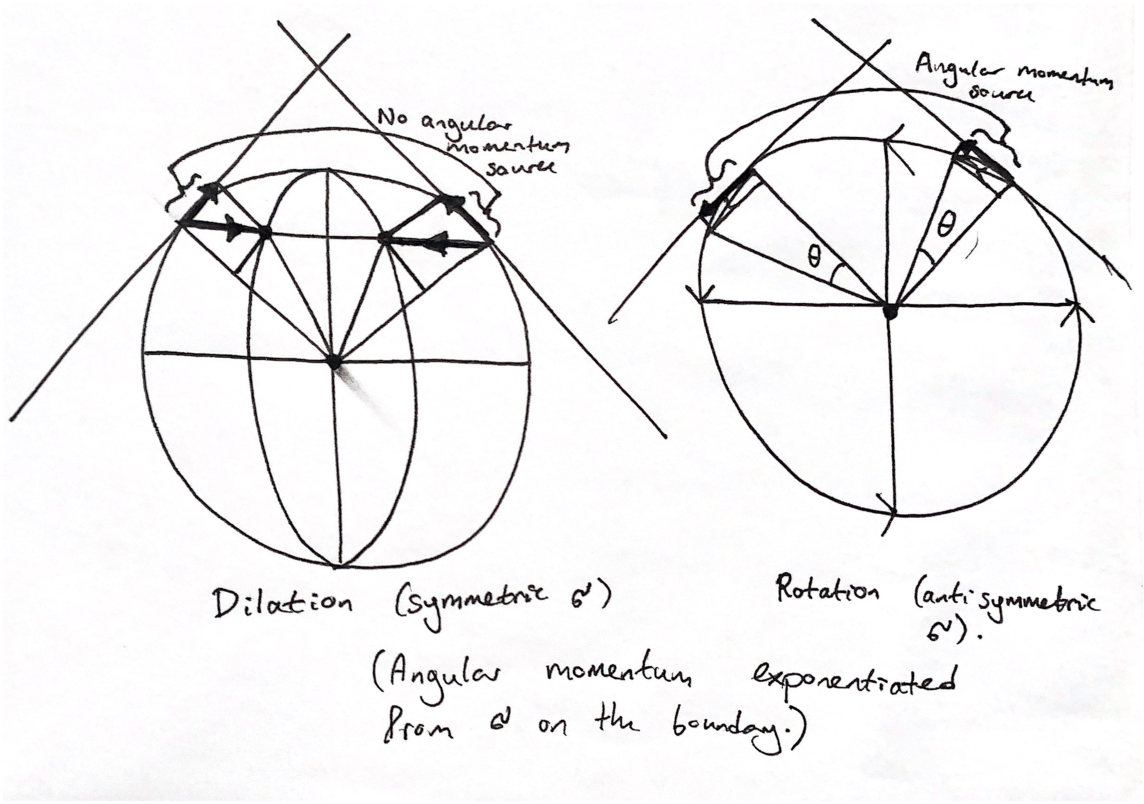
\includegraphics[page=1,width=0.7\linewidth]{figures/3.pdf}
% \end{center}


% If the control volume follows the flow, the Reynolds transport theorem \eqref{reynolds_transport_theorem} gives a rate of change of angular momentum:
% \begin{equation}\label{moment_of_linear_momentum_reynolds}
%     \frac{d}{dt}\eval{\left[\int_{\omn(t)} \bar{x} \wedge \left(\rho u\right)\,dx\right]}_{t=0}
%     % = \int_{\omn(0)} \left(x - c\right)\wedge \left(\rho g\right)\,dx + \int_{\pomn(0)} \left(x - c\right) \wedge \hat
%     = \int_{\omn(0)} \bar{x} \wedge \Part{(\rho u)}{t}\,dx + \int_{\pomn(0)} \bar{x} \wedge \rho u (u\cdot \hat{n})\,dx.
% \end{equation}
% The source terms of linear momentum are body forces $\rho g$ on the interior and tractions $\hat{t}$ on the boundary.
% Therefore we have an explicit equation for the rate of change of angular momentum, which we equate to the right-hand-side of
% \eqref{moment_of_linear_momentum_reynolds}:
% \begin{equation}\label{moment_of_linear_momentum_sources}
%     \int_{\omn(0)} \bar{x} \wedge \Part{(\rho u)}{t}\,dx + \int_{\pomn(0)} \bar{x} \wedge \rho u (u\cdot \hat{n})\,dx
%     = \int_{\omn(0)} \bar{x} \wedge \left(\rho g\right)\,dx + \int_{\pomn(0)} \bar{x} \wedge \left(\sigma \hat{n}\right)\,dx.
% \end{equation}
% By the Euler-Cauchy stress principle (section \ref{stress_principle}), we have let the traction $\hat{t} = \sigma \hat{n}$.
% For comparison, we repeat here an integral form of linear momentum conservation, which already must hold:
% \begin{equation*}
%     \int_{\omn(0)} \Part{(\rho u)}{t}\,dx + \int_{\pomn(0)} \rho u (u\cdot \hat{n})\,dx
%     = \int_{\omn(0)} \left(\rho g\right)\,dx + \int_{\pomn(0)} \sigma \hat{n}\,dx.
% \end{equation*}
% >>>
% >>>

\subsection{Conservation of energy}
% <<<
\begin{equation*}
\begin{split}
    \frac{D\rho}{Dt} + \rho\nabla\cdot u = 0 &\quad\text{(Conservation of mass)},\\
    \rho\frac{Du}{Dt} = \rho g + \nabla\cdot\sigma &\quad\text{(Conservation of linear momentum)},\\
    \sigma = \sigma^T &\quad\text{(Conservation of angular momentum)}.
\end{split}
\end{equation*}
% >>>

\section{Scaling and dimension}
% <<<
\subsection{The Reynolds number}
% >>>

\section{Stokes flow and the meaning of pressure}\label{pressure_derivation}
% <<<
If we assume that the advective term $u\cdot \nabla u$ in the incompressible Navier-Stokes equations is ``small'',
we can ignore it and derive the linear \textit{unsteady Stokes equations}:
\begin{equation}\label{unsteady_stokes}
    \rho\Part{u}{t} = \mu\Delta u + \rho g - \nabla p, \quad \nabla\cdot u = 0.
\end{equation}
We are assuming validity for low Reynolds number $Re \ll 1$, where convective behaviour is neglible compared to the viscous forces, which for a
Navier-Stokes fluid ``diffuse'' the linear momentum. Setting the left-hand-side of \eqref{unsteady_stokes} to zero results in the \textit{steady Stokes equations}
\begin{equation}\label{steady_stokes}
    \mu\Delta u + \rho g - \nabla p = 0,\quad \nabla\cdot u = 0.
\end{equation}
Time-dependent equation \eqref{unsteady_stokes} can be thought of as a ``gradient descent'' to find the steady Stokes flow \eqref{steady_stokes}.
The steady Stokes equation is a constrained vector Poisson equation, where we have introduced pressure $p$ explicitly.
It is well-known, by Dirichlet's principle, that we can think
of a weak solution to the unconstrained vector Poisson equation as a minimiser of the Dirichlet energy,
\begin{equation}
\begin{aligned}
& \underset{u}{\text{minimize}}
& & E(u) =  \frac{\mu}{2} \inner{\nabla u, \nabla u} - \inner{u, \rho g}.\\
\end{aligned}
\end{equation}
\newcommand{\energygradient}{\frac{\delta E}{\delta u}}
We can validate this by computing the Euler-Lagrange equations:
\begin{align*}
    % \frac{\delta E}{\delta u} = \Part{\fancyL}{u} - \frac{d}{dx}\Part{\fancyL}{\nabla u}
    % notation?
    \frac{\delta E}{\delta u} = \Part{\fancyL}{u} - \frac{d}{dx}\Part{\fancyL}{u_x}
                              = -\rho g - \mu\Delta u = 0.
\end{align*}
We now introduce the incompressibility constraint $\nabla \cdot u = 0$, giving the constrained minimization
\begin{equation}\label{stokes_flow_optimization}
\begin{aligned}
& \underset{u}{\text{minimize}}
& & E(u) =  \frac{\mu}{2} \inner{\nabla u, \nabla u} - \inner{u, \rho g}\\
& \text{subject to}
& & \nabla\cdot u = 0.
\end{aligned}
\end{equation}
It is not immediately obvious how to form the constrained Euler-Lagrange equations here, as $\nabla\cdot$ is a differential operator.
We cannot just write
    $$\text{``}\frac{\delta E}{\delta u} = \lambda\nabla\cdot\text{''}$$
for scalar function $\lambda$, as we can with a pointwise linear constraint such as $u\cdot v = 0$ for some vector field $v$. However, this is just a problem of
notation. The evaluation of energy change with perturbations is defined as
\begin{align*}
    \inner{\frac{\delta E}{\delta u}, \delta u} = \int_\Omega \frac{\delta E}{\delta u}\cdot\delta u\,dx.
\end{align*}
We want this measure of energy change to be purely a divergence measure, up to a scalar multiplier $\lambda$:
\begin{equation}\label{el_pressure_constrained_div}
    \int_\Omega \frac{\delta E}{\delta u}\cdot\delta u\,dx = \int_\om \lambda \nabla\cdot \delta u\,dx.
\end{equation}
This means
that virtual displacements with $\nabla\cdot\delta u = 0$ will not cause an energy change, which is the condition that
we want for a stationary point.
We can now apply integration by parts to \eqref{el_pressure_constrained_div}, assuming that $\delta u$ vanishes on the boundary of the domain, to get
\begin{equation}
    \int_\Omega \frac{\delta E}{\delta u}\cdot\delta u\,dx = -\int_\om \nabla\lambda \cdot \delta u\,dx.
\end{equation}
We can now reasonably apply the localisation step to get the constrained Euler-Lagrange equations
\begin{equation}
\begin{split}
           \frac{\delta E}{\delta u} = -\nabla \lambda
    \quad\equiv\quad \mu\Delta u + \rho g - \nabla \lambda = 0.
\end{split}
\end{equation}
Along with the constraint $\nabla\cdot u = 0$, this is just the steady Stokes equations \eqref{steady_stokes}, where $\lambda = p$! We can see that the pressure $p$
is actually
a Lagrange multiplier, which measures a virtual force that responds to virtual displacements which would break the constraint of incompressibility.
In fact, we may think of this as a derivation of the pressure.

\subsubsection{Alternative direct derivation in terms of a modified energy}
Previously, we emphasized the meaning of the Lagrange multiplier. One utility of Lagrange's methods is their automated calculational power.
It is standard to express that a solution to the optimization
problem \eqref{stokes_flow_optimization}, with a differentiable equality constraint, is a stationary point of the modified energy
\begin{equation}\label{stokes_flow_modified_energy}
    L(u, \lambda) \coloneqq \frac{\mu}{2} \inner{\nabla u, \nabla u} - \inner{u, \rho g} - \inner{\lambda, \nabla\cdot u}.\\
\end{equation}
We can take an evaluated first variation with respect to $u$ to get
\begin{align*}
    \inner{\frac{\delta L}{\delta u}, \delta u} = \inner{-\rho g - \mu\Delta u, \delta u} - \inner{\lambda, \nabla\cdot\delta u},
\end{align*}
which by integration by parts becomes
\begin{equation}
    \inner{\frac{\delta L}{\delta u}, \delta u} = \inner{-\rho g - \mu\Delta u + \nabla \lambda, \delta u}.
\end{equation}
We then get
\begin{equation}
\begin{split}
    \frac{\delta L}{\delta u} &= -\rho g - \mu\Delta u + \nabla \lambda = 0,\\
    \frac{\delta L}{\delta \lambda} &= -\nabla\cdot u = 0,
\end{split}
\end{equation}
which are the steady Stokes equations \eqref{steady_stokes} with pressure $p = \lambda$.



\subsection{Application to hydrostatics}
For example, we may imagine the steady Stokes equations modelling a calm sea with a flat seabed.
We can let the body force be gravity described by a potential $\phi$:
    $$\rho g = -\nabla \phi.$$
If we make a perturbed displacement of the velocity field at the bottom of the ocean, supposing that some volume of water
is beginning to expand,
we are working against gravity as well as our virtual force, pressure.

\vskip 0.2in
(draw this)
\vskip 0.2in

% >>>

% \subsection{Kinds of fluids}
% \subsubsection{Incompressible fluids}
% \subsubsection{Inviscid flow}
% \subsubsection{Irrotational flow}
% \subsubsection{Steady flow}
% \subsubsection{Viscous flow and Newtonian fluids}



\chapter{Two Galerkin methods for Poisson's equation}
% The Finite Element Method

\section{Introduction}

Continuum mechanics provides the foundation for understanding of fluid motion, and the Navier-Stokes equations for
a Newtonian fluid are the primary model for the prediction of fluid behaviour in engineering.
The domain and initial/boundary conditions can be arbitrarily complex. For example, fluid motion is often simulated
through a digital surface model of a real-world object or system created in computer-aided design software.
On the other side of the coin, fluid models are very often used in modern film, both live-action and animated.

The Navier-Stokes equations in applications are primarily
solved on a computer, and a computer works with both finite data and finite precision. The Galerkin method
is particularly amenable to computer implementation, so much so that the whole process of geometric modelling, boundary condition handling,
residual minimisation, and solution reconstruction, can be automated (\cite{fenics_book}, \cite{DOLFIN}). We begin by discussing
possibly the simplest instance of a Galerkin method, performed on an irregular 2D domain to emphasize that the method trivially extends
to complex geometries. A computer implementation is then presented, which generates visualisations and quality metrics for the results.

\captionsetup[subfigure]{labelformat=empty}
\begin{figure}[H]
    \centering
    \subfloat[][\centering Peter Dirichlet (1805--1859)]{{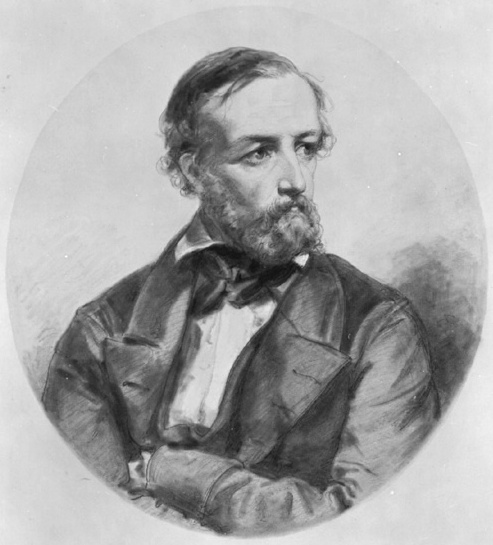
\includegraphics[height=3cm]{figures/mathematicians/Peter_Dirichlet.jpg} }}
    \qquad
    \subfloat[][\centering David Hilbert (1862--1943)]{{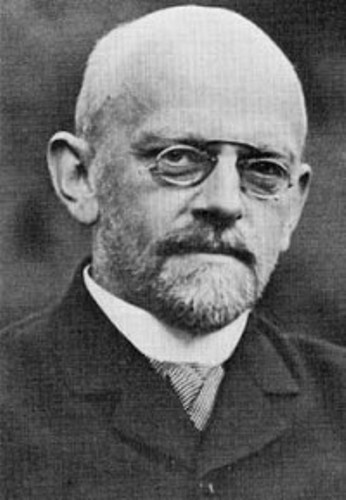
\includegraphics[height=3cm]{figures/mathematicians/David_Hilbert.jpeg} }}
    \qquad
    \subfloat[][\centering Walther Ritz (1878--1909)]{{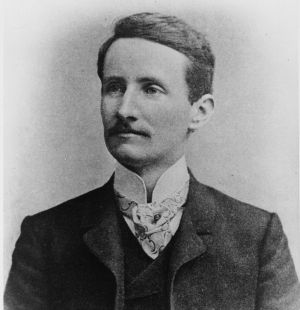
\includegraphics[height=3cm]{figures/mathematicians/Walther_Ritz.jpg} }}
    \qquad
    \subfloat[][\centering Boris Galerkin (1871--1945)]{{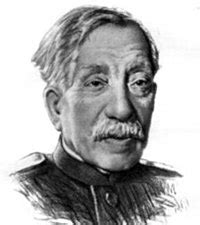
\includegraphics[height=3cm]{figures/mathematicians/Boris_Galerkin.jpeg} }}
    \qquad
    \subfloat[][\centering Sergei Sobolev (1908--1989)]{{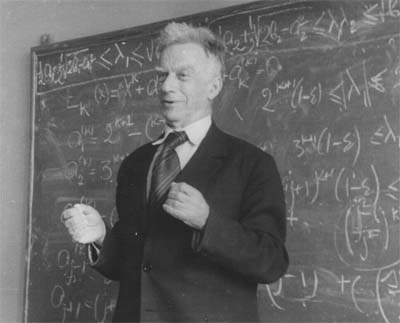
\includegraphics[height=3.5cm]{figures/mathematicians/Sergei_Sobolev.jpg} }}
    \qquad
    \subfloat[][\centering Laurent Schwartz (1915--2002)]{{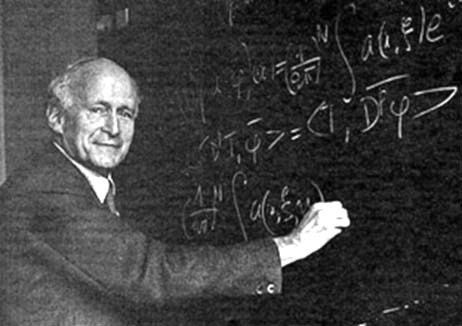
\includegraphics[height=3.5cm]{figures/mathematicians/Laurent_Schwartz.jpeg} }}
    \caption{Some key figures whose work precipitated modern developments in PDEs.}
    \label{fig:galerkin_mathematicians}
\end{figure}


\subsubsection{The Galerkin method}
The Galerkin method was established by engineer and mathematician Boris Galerkin (1871--1945) in a 1915 paper containing
an approximation method for the biharmonic equation of classical beam theory \cite{boris_galerkin}. Briefly, the principle of Galerkin is to
choose a space of approximations, today called ``test functions'', and solve for the test function which minimises a residual error with respect
to some function space norm. This norm is induced by a choice of what are now called the ``trial functions''. If the trial functions are the same as the test functions,
the residual is minimised with respect to the Euclidean norm.

% \renewcommand\thesubfigure{}
% \begin{figure}[H]
%     \centering
%     \footnotesize
%     \stackunder[5pt]{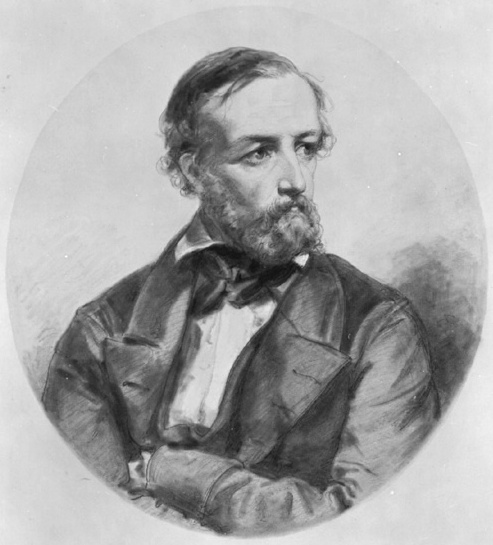
\includegraphics[width=2.5cm]{figures/mathematicians/Peter_Dirichlet}}{Peter Gustav Lejeune Dirichlet (1805--1859)}
% 
%     \footnotesize
%     \stackunder[5pt]{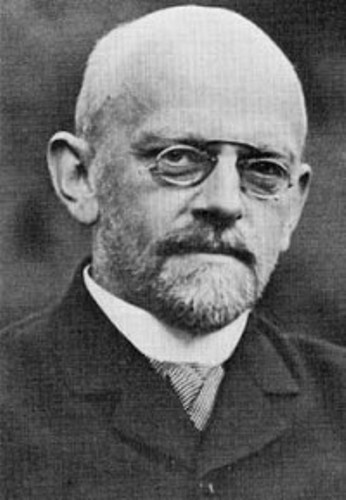
\includegraphics[width=2.5cm]{figures/mathematicians/David_Hilbert.jpeg}}{David Hilbert (1862--1943)}
% 
%     \footnotesize
%     \stackunder[5pt]{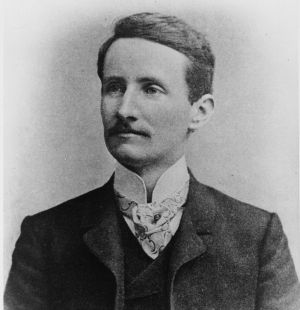
\includegraphics[width=2.5cm]{figures/mathematicians/Walther_Ritz.jpg}}{Walther Ritz (1878--1909)}
% 
%     \footnotesize
%     \stackunder[5pt]{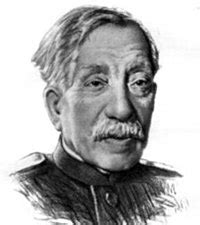
\includegraphics[width=2.5cm]{figures/mathematicians/Boris_Galerkin.jpeg}}{Boris Galerkin (1871--1945)}
% 
%     \footnotesize
%     \stackunder[5pt]{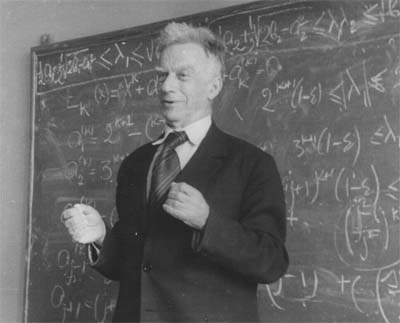
\includegraphics[width=2.5cm]{figures/mathematicians/Sergei_Sobolev.jpg}}{Sergei L. Sobolev (1908--1989)}
% 
%     \footnotesize
%     \stackunder[5pt]{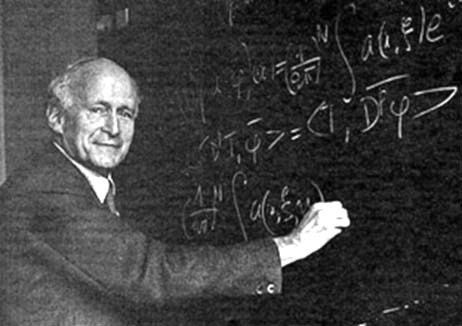
\includegraphics[width=2.5cm]{figures/mathematicians/Laurent_Schwartz.jpeg}}{Laurent Schwartz (1915--2002)}
% 
%     \label{fig:example}
% \end{figure}

As well as proving highly useful
in numerical applications, the methods of Galerkin (and contemporary mathematicians such as Walther Ritz) precede important developments
in the mathematical theory of PDEs. In a 1934 talk named ``Generalized Solutions to the Wave Equation'', mathematician Sergei L. Sobolev (1908--1989)
precipitated the development
of generalised functions by Laurent Schwartz (1915-2002), integral to the modern study of PDEs
(\cite{sobolev_web_page}, \cite{one_hundred_years_galerkin}).
These developments are clarifications on the question: What do we mean when we speak of a solution of a PDE from physics? Galerkin's method
is much closer to the answer than, for example, the finite difference method.


\subsubsection{The finite element method}

\subsubsection{The Poisson equation}

Among the fundamental PDEs
are the heat equation
    $$\Part{h}{t} = \Delta h + g$$
and the Poisson equation
\begin{equation}\label{poisson_compact}
    -\Delta h = g.
\end{equation}
The latter can be thought of as the steady-state version of the former. The solution of a Poisson problem will be a crucial component
of the solution of the Stokes equations. It seems ideal to start by discussing
discretization methods for the Poisson equation \eqref{poisson_compact} in particular,
as it is likely the simplest non-trivial PDE.
The focus here is on the Dirichlet problem
\begin{equation}\label{poisson_dirichlet_problem}
    -\Delta h = g, \quad \left.h\right|_{\Gamma} = h_\Gamma,
\end{equation}
where $\Gamma$ is the boundary of the domain, and the domain is 2D.

\section{Discretizing the differential versus integral form}
\subsection{Discretizing the differential form of the PDE}
It is a theorem of Gauss that in Euclidean space $\mathbb{R}^3$ we have
\begin{equation}\label{gauss_euclidean_divergence}
    \nabla \cdot v = \Part{v_x}{x} + \Part{v_y}{y} + \Part{v_z}{z},
\end{equation}
and we get \eqref{poisson_compact} in the form
\begin{equation}\label{poisson_differential_intro}
    -\left(\frac{\partial^2 h}{\partial x^2}
           +\frac{\partial^2 h}{\partial y^2}
           +\frac{\partial^2 h}{\partial z^2}\right) = g.
\end{equation}
Thinking about \eqref{poisson_differential_intro} leads to the finite difference method, historically the first and
still very important in applications.
By forming secant approximations of the derivatives over a regular grid, a linear system is formed, and the approximate solution is solved
for as a function of this grid.
However, it may be hard to give a real interpretation of what the solution samples at grid points say about the solution everywhere.
They could be coefficients of, for example, hat basis functions.
Yet a finite difference discretization of the Poisson equation \eqref{poisson_compact} may not take this into account at all. One might feel that
limits have been taken too soon.

% Consider a single conservation law as described in section \ref{conservation_laws}. This law
% was given in two forms, ``integral'' \eqref{continuity_equation}:
% \begin{equation*}
%     \frac{d}{dt} \int_{\Omega_0} \phi\,dx = \int_{\Omega_0} s\,dx + \int_{\pomn} \phi j \cdot \left(-\hat{n}\right)\,dx,
% \end{equation*}
% and ``differential'' \eqref{continuity_equation_differential}:
% \begin{equation*}
%     \Part{\phi}{t} = s - \nabla\cdot (\phi j).
% \end{equation*}

\subsection{Discretizing the integral form of the PDE}
In physics, Poisson's equation is an equilibrium conservation law, and therefore has an integral form.
This form will give clearer routes to discretizations which
have geometric meaning.
% Thinking instead about \eqref{poisson_integral_intro} will lead to Galerkin methods, which include finite volumes, finite elements, and spectral methods.
For example, the general integral conservation law \eqref{continuity_equation},
\begin{align*}
    \frac{d}{dt} \int_{\Omega_0} \phi\,dx = \int_{\Omega_0} s\,dx + \int_{\pomn} \phi j \cdot \left(-\hat{n}\right)\,dx,
\end{align*}
is a geometric statement about fluxes
of quantity $\phi$ by $j$, quantified over arbitrary control volumes $\Omega_0$.
There are an infinite number of control volumes, and therefore an infinite number of equations which must hold, and there is an infinite-dimensional
space of solutions to choose from. A key idea, then, is to choose a finite number of equations and a finite-dimensional subspace of possible approximate solutions.
A supposed solution will be represented by the coefficients of some choice of basis functions for the subspace. Each equation will be checked exactly against this supposed solution.

\vskip 0.2in
(figure)
\vskip 0.2in

Finite element methods, and more generally Galerkin methods, live comfortably in the language of weak solutions, integral forms of partial differential equations,
and the calculus of variations.
To continue with this idea, we must write the Poisson equation \eqref{poisson_compact} in integral form.

\section{Deriving the heat and Poisson equation through diffusion processes}
The Poisson equation \eqref{poisson_compact} can be thought of as the steady state of some diffusion process with a source term $g$,
although this need not be its literal physical interpretation.
A diffusion process ``levels out'' some quantity, such as temperature or some chemical concentration.
A diffusion could intuitively be thought of as a
progressive ``blurring'',
such as in a camera defocus, and in fact many common image processing techniques use diffusion PDEs from physics \cite{tum}. We will stick with
the notion of ``temperature'' $h$ as the diffused quantity.
\textit{Fick's law of diffusion} is a constitutive relation giving the bulk flux of temperature $h$ as proportional to the negative gradient:
    $$hj = -\mu\nabla h,$$
where $\mu$ is called the diffusion coefficient.
This is one way of saying that the temperature tends to level out.
If we form a continuity equation \eqref{continuity_equation} for temperature, with source $s$, we get
\begin{equation}\label{heat_equation_integral}
    \frac{d}{dt} \int_{\Omega_0} h\,dx = \int_{\Omega_0} s\,dx + \int_{\pomn} \mu \nabla h \cdot \hat{n}\,dx,
\end{equation}
which by application of Stokes' theorem becomes
\begin{equation}\label{heat_equation_differential}
    \frac{dh}{dt} = s + \nabla \cdot \left(\mu \nabla h\right).
\end{equation}
If we further assume that the diffusion coefficient $\mu$ is constant, we get
\begin{equation}\label{heat_equation_differential_constant}
    \frac{dh}{dt} = s + \mu\nabla \cdot \nabla h = s + \mu\Delta h,
\end{equation}
which is the standard heat equation.
The steady-state heat equation is then
\begin{equation}\label{poisson_equation}
    -\Delta h = g,
\end{equation}
where we let $g = s/\mu$ in the above.
This completes the derivation of the Poisson equation \eqref{poisson_compact}.
% which models steady-state diffusion processes and can be used to calculate gravitational or electrostatic potential fields.
In integral form, ``undoing'' the application of Stokes' theorem above, the Poisson equation is
\begin{equation}\label{poisson_equation_integral}
    \int_{\pomn} -\nabla h\cdot \hat{n}\,dx = \int_{\omn} g\,dx \quad \text{for all control volumes $\Omega_0$.}
\end{equation}
Form \eqref{poisson_equation_integral} clearly shows that we are calculating a steady state,
as we are solving for $h$ such that the amount of heat that leaves $\Omega_0$ is the amount introduced into $\Omega_0$ by the source function.
The form \eqref{poisson_equation_integral}, rather than \eqref{poisson_compact}, will be the starting point for deriving Galerkin methods.

\section{Discretizing Poisson's equation by finite volumes}\label{discretizing_poisson}

Equation \eqref{poisson_equation_integral} is quantified over an infinite number of control volumes $\Omega_0$.
These control volumes are in the interior of $\Omega$, as the solution at the boundary $\Gamma$ is specified by the Dirichlet boundary condition
$\left.h\right|_\Gamma = h_\Gamma$, and there is no flux information across $\Gamma$.
A simple idea is to choose a finite number of control volumes $\Omega_1,\cdots,\Omega_n$ (hence ``finite volumes''), and check that the flux integral holds over each of these.
We will then have $n$ equations on $h$. As this system will be underdetermined ($h$ has infinite degrees of freedom), we must
restrict $h$ to a finite-dimensional space of approximations $\Phi^*$.


\subsection{The Dirichlet boundary condition and the test space}
The solution is completely known on $\Gamma$ by the Dirichlet boundary condition $\left.h\right|_\Gamma = h_\Gamma$.
However, the finite dimensional space $\Phi^*$ may not be able to exactly represent the boundary function $h_\Gamma$,
and therefore the first step is to approximate $h_\Gamma$ (for which there are many options, for example
projection in the $L^2$-norm or interpolation across a finite sampling of boundary points \cite{approximation_theory}). Choosing some $\phi_\Gamma \in \Phi^*$ with
    $$\left.\phi_\Gamma\right|_\Gamma \approx h_\Gamma,$$
we can define an ``interior'' function space
$$
    \Phi = \left\{h^* \in \Phi^* \mid \left.h\right|_\Gamma = 0 \right\},
$$
and the approximate solution $\tilde{h}$ will then be
$$
    \tilde{h} = \phi + \phi_\Gamma
$$
for some $\phi \in \Phi$.
In the finite volume and finite element literature the space $\Phi$ is called the test space.
Since we selected $n$ control volumes $\Omega_1,\cdots,\Omega_n$, the approximating space $\Phi^*$ must be chosen such that
$\Phi$ is $n$-dimensional. We can choose a basis for the test space,
    $$\Phi = \text{span}\left\{\phi_1,\cdots,\phi_n\right\}.$$
The problem is now to find a vector of coefficients of these test functions,
    $\hat{h} = (h_1, \cdots, h_n)^T,$
and reconstruct the solution as
    $$\tilde{h} = \phi + \phi_\Gamma,$$
where $\phi$ is the ``interior variation''
    $$\phi = \Phi\cdot \hat{h} \coloneqq h_1\phi_1 + \cdots + h_n\phi_n.$$

\subsection{Forming a linear system}
The integral-conservation-law form \eqref{poisson_equation_integral} of the Poisson equation \eqref{poisson_compact}
now directly indicates a method of approximation. Letting $h$ be approximated by $\tilde{h} = \phi + \phi_\Gamma$ (where $\phi \in \Phi$ is unknown and $\phi_\Gamma \in \Phi^*$ is known),
and restricting the flux integrals to the control volumes $\Omega_1,\cdots,\Omega_n$, the conservation law \eqref{poisson_equation_integral} becomes
\begin{equation}\label{poisson_equation_integral_fvm}
    \int_{\partial\Omega_j} -\nabla \left(\phi + \phi_\Gamma\right) \cdot \hat{n}\,dx = \int_{\Omega_j} g\,dx \quad\quad j=1,\cdots,n.
\end{equation}
The ``interior variation'' $\phi = \Phi\cdot \hat{h}$ is the only unknown, so we can move all knowns to the right-hand-side
and expand $\phi$ in terms of the basis test functions $\phi_1,\cdots,\phi_n$:
\begin{equation}\label{poisson_equation_integral_fvm_knowns_unknowns}
    \int_{\partial\Omega_j} -\nabla \left(\sum_{i=1}^nh_i\phi_i\right) \cdot \hat{n}\,dx =
            \int_{\Omega_j} g\,dx
            + \int_{\partial\Omega_j} \nabla \phi_\Gamma \cdot \hat{n}\,dx
 \quad\quad j=1,\cdots,n.
\end{equation}
By linearity, to emphasize the separate integrals that need to be computed, the above equation can be written as
\begin{equation}\label{poisson_equation_integral_discretized}
    \sum_{i=1}^n h_i\int_{\pom_j} -\nabla \phi_i \cdot \hat{n}\,dx =
            \int_{\Omega_j} g\,dx
            + \int_{\partial\Omega_j} \nabla \phi_\Gamma \cdot \hat{n}\,dx
 \quad\quad j=1,\cdots,n.
\end{equation}
It is seen here that there must be some restrictions on the $\phi_i$ and $\phi_\Gamma$.
Formally, they must be in the Sobolev space $H^1(\Omega)$. This simply means that they must have a gradient defined ``almost everywhere''.
It does not matter if the gradient is not defined at isolated lower-dimensional subsets, as these make no contribution to
the integral. The system \eqref{poisson_equation_integral_discretized} can be written in matrix form as
\newcommand{\integralentry}[2]{\int_{\pom_{#1}}-\nabla\phi_{#2}\cdot\hat{n}\,dx}
\newcommand{\integralrhsentry}[1]{\int_{\om_{#1}}g\,dx + \int_{\pom_{#1}}\nabla\phi_\Gamma\cdot\hat{n}\,dx}
\begin{equation}\label{poisson_matrix_equation}
\begin{split}
    A\hat{h}
    &= \begin{bmatrix}
            \integralentry{1}{1} & \cdots & \integralentry{1}{n} \\
            \vdots & & \vdots \\
            \integralentry{n}{1} & \cdots & \integralentry{n}{n}
    \end{bmatrix}
    \begin{bmatrix} h_1 \\ \vdots \\ h_n \end{bmatrix}
    \\
    &= \begin{bmatrix} \integralrhsentry{1} \\ \vdots \\ \integralrhsentry{n}  \end{bmatrix}
    = \hat{f}.
\end{split}
\end{equation}
This system is solved for the coefficients of combination for the test functions, $\hat{h} = h_1 \cdots h_n)^T$, and the approximate
solution is constructed as $\tilde{h} = \Phi\cdot\hat{h} + \phi_\Gamma$.
If the domain partition $\Omega_1,\cdots,\Omega_n$ and test space $\Phi = \text{span}\left\{\phi_1,\cdots,\phi_n\right\}$
are chosen well, this linear system will be non-singular and hopefully well-conditioned.
In all cases we have a conservative system of balanced fluxes, but it is another question whether the approximation
$\tilde{h}$ is good.

\subsection{Choosing the test space, boundary approximation, and control volumes}
Possibly the simplest scheme is to triangulate $\Omega$ as
    $\bigcup_i T_i,$
such that we have $n$ interior vertices $p_1,\cdots,p_n$, and $n_\Gamma$ boundary vertices $p^\Gamma_1,\cdots,p^\Gamma_{n_\Gamma}$, and $n_T$ triangles
$T_1,\cdots,T_{n_T}$.

\subsubsection{The test space}
Firstly, there is a clear choice of function space $\Phi^*$, which satisfies the $H^1$ condition, consisting of piecewise linear ``hat'' basis functions
at each interior or boundary vertex,
\newcommand{\hatfun}[1]{\text{Hat}(#1)}
$$
    \Phi^* = \text{span}\left\{
        \hatfun{p_1},\cdots,\hatfun{p_n},
        \hatfun{p^\Gamma_1},\cdots,\hatfun{p^\Gamma_{n_\Gamma}}
    \right\}.
$$
The hat function at a vertex has value $1$ at that vertex and value $0$ at its neighbours.
The test space (which is zero on the boundary $\Gamma$) is then
$$
    \Phi = \text{span}\left\{
        \hatfun{p_1},\cdots,\hatfun{p_n}
    \right\} = \text{span}\left\{\phi_1,\cdots,\phi_n\right\}.
$$
An example decomposition for an ellipse-shaped domain is shown in figure \ref{ellipse_partition}.
\begin{figure}[H]
    \begin{center}
        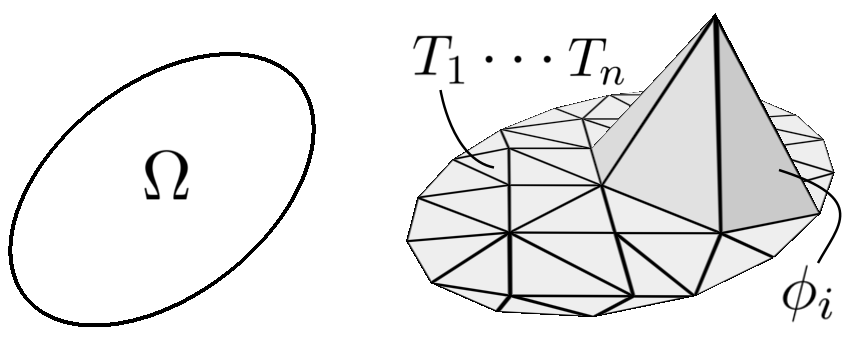
\includegraphics[width=0.53\linewidth]{figures/hat.png}
    \end{center}
    \caption{\scriptsize
        The domain $\Omega$ is partitioned into triangular cells $T_1\cdots T_{n_T}$. One example of a hat basis function $\phi_i$ is shown, where
        the vertical axis is the basis function value.
    }
    \label{ellipse_partition}
\end{figure}

\subsubsection{Approximating the boundary values}
One simple approximation of $\left.h\right|_\Gamma = h_\Gamma$ is
$$
    \phi_\Gamma = h_\Gamma(p^\Gamma_1)\hatfun{p^\Gamma_1}
                + \cdots
                + h_\Gamma(p^\Gamma_{n_\Gamma})\hatfun{p^\Gamma_{n_\Gamma}},
$$
which is a piecewise linear interpolation when restricted to the boundary $\Gamma$. The approximation $\phi_\Gamma$ for some boundary
function $h_\Gamma$ is shown in figure \ref{boundary}.
\begin{figure}[H]
    \begin{center}
        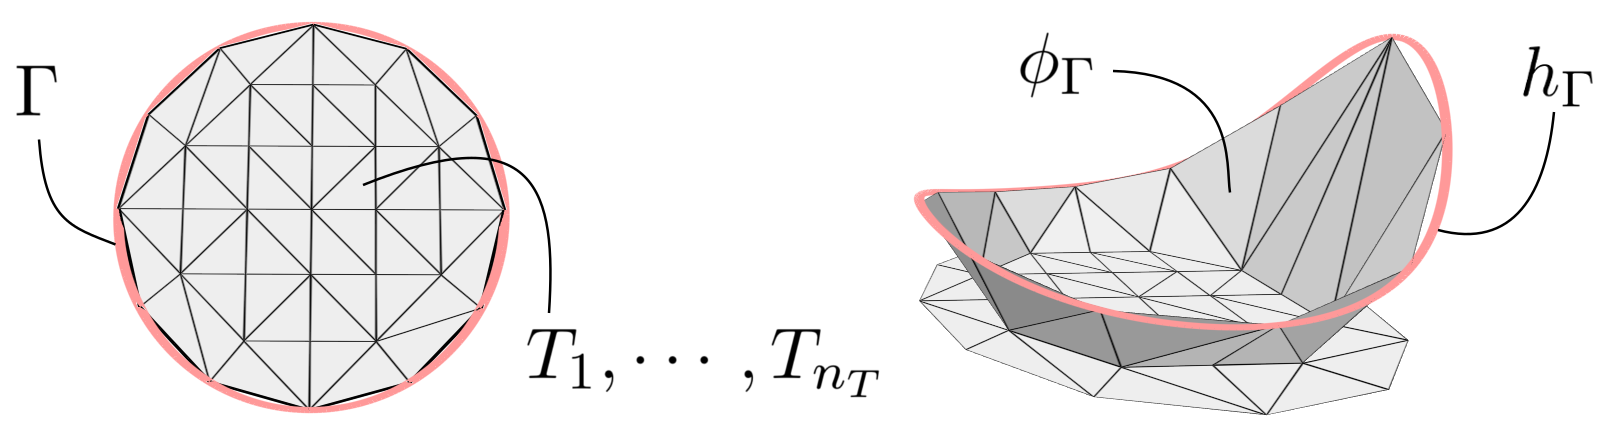
\includegraphics[width=0.9\linewidth]{figures/boundary/boundary.png}
    \end{center}
    \caption{\scriptsize
        A circle domain $\Omega$ with boundary $\Gamma$ is tessellated by triangles $T_1,\cdots,T_{n_T}$.
        The boundary function $h_\Gamma$ is approximated by $\phi_\Gamma$, a linear combination of hat functions centred at the boundary vertices.
    }
    \label{boundary}
\end{figure}

\subsubsection{Choosing a finite number of control volumes}
If we choose some characteristic ``triangle centre'' for each triangle, then we can associate to the interior vertices
$p_1,\cdots,p_n$ a set of domains $\Omega_1,\cdots,\Omega_n$. Each $\Omega_i$ is defined by the polygon which joins the centres of the triangles
incident to $p_i$.
Two common choices for the triangle centre are the barycentre, which is the average position of the three vertices, and the circumcentre,
which is the centre of the unique circle passing through the three vertices. The circumcentre scheme gives what are called
``Voronoi cells'' due to their relation to Voronoi diagrams in computational geometry \cite{orourke}.
The resulting cell decompositions are displayed in figure
\ref{cell_decompositions}.

\begin{figure}[H]
    \begin{center}
        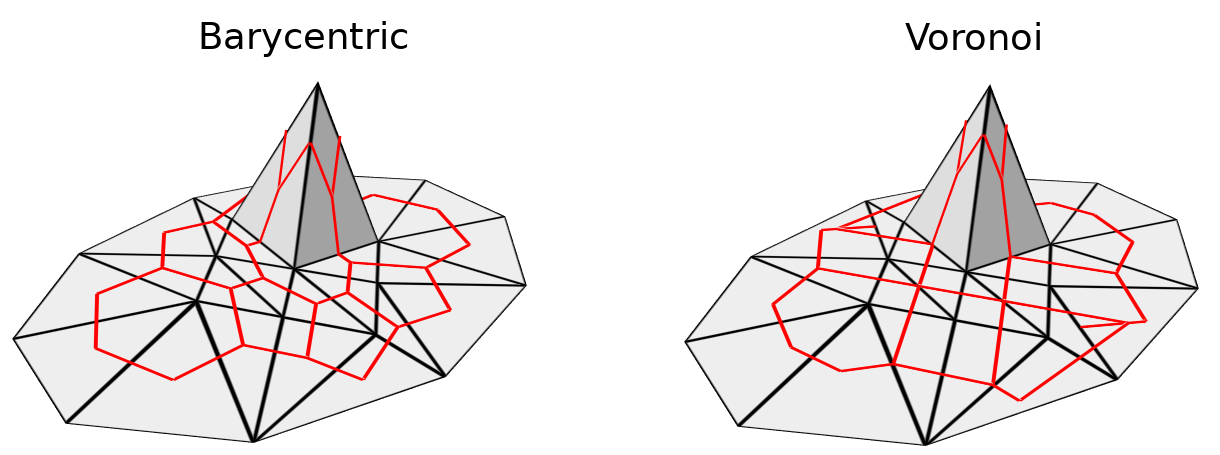
\includegraphics[width=0.7\linewidth]{figures/cell.png}
    \end{center}
    \caption{\scriptsize
        The domain $\Omega$ is partitioned into triangular cells $T_1\cdots T_{n_T}$.
        Flux integrals are taken over $n$ polygonal cells, one for each internal vertex $p_i$, for example using triangle barycenters or circumcenters.
    }
    \label{cell_decompositions}
\end{figure}

This scheme has found some success, especially in the domain of geometry processing \cite{polygon_mesh_processing}.
By Stokes' theorem, the matrix $A$ in \eqref{poisson_matrix_equation} can be thought of as a negative discrete Laplacian.
If we compute these integrals, we will find a very simple closed form for the entries of $A$:

$$\text{cotan formula.}$$

In geometry processing this matrix is called the ``cotangent Laplacian'' \cite{polygon_mesh_processing}, and it is typically
applied to surface meshes in $\mathbb{R}^3$, which can be thought of as triangulations of a smooth surface.

\subsection{Results and visualisation}
\vskip 0.2in
(results and visualisation)
\vskip 0.2in
We have worked through an instance of a \textit{finite volume method} \cite{pde_larsson}.
Finite volume methods are characterised by an exact domain partition and computation of flux integrals.
Finite volume methods are typically \textit{conservative}, due to the ``flux network'' nature of the discretisation.
\section{From finite volumes to finite elements}\label{trial_function}
The alternative ``finite element'' approach is directly related to the ``finite volumes'' described above. While each finite volume
had a direct geometric meaning (as a small cell in which a certain test flux integral is taken), the geometric meaning of a ``finite element''
requires slightly more thought, although it will be seen to be the same idea in disguise.
The matrix equation \eqref{poisson_matrix_equation} consists of linear equations
\begin{align*}
    \int_{\pom_1} -\nabla \left(\sum_{i=1}^n h_i\phi_i\right) \cdot \hat{n}\,dx
    =
    \int_{\om_1}g\,dx\quad\text{(for $j=1$)},
\end{align*}
and so on. We cannot compute flux integrals
over all arbitrary control volumes, but we can take a number of ``trial'' flux integrals over the finite number of cells $\Omega_i$.
We can take linear combinations of these equations to get more equations which must hold on a solution.
For example,
\begin{equation}\label{example_trial_sum}
    \int_{\pom_1} -\nabla \left(\sum_{i=1}^n h_i\phi_i\right) \cdot \hat{n}\,dx
    +
    \int_{\pom_2} -\nabla \left(\sum_{i=1}^n h_i\phi_i\right) \cdot \hat{n}\,dx
    =
    \int_{\om_1}g\,dx
    +
    \int_{\om_2}g\,dx
\end{equation}
must hold. At first sight, \eqref{example_trial_sum} cannot directly be interpreted as a statement about a ``flux integral'', but rather about a sum
of flux integrals. However, a key idea is to regard \eqref{example_trial_sum} as a flux integral over a \textit{formal sum} of domains,
    $$\Omega_1 + \Omega_2.$$
We now have the equation
\begin{equation}
    \int_{\pom_1 + \pom_2} -\nabla \left(\sum_{i=1}^n h_i\phi_i\right) \cdot \hat{n}\,dx
    =
    \int_{\om_1 + \om_2}g\,dx.
\end{equation}
In differential geometry $\Omega_1 + \Omega_2$ is called a \textit{chain}. For example, we may visualise $\Omega_1 + 2\Omega_2 + 0.5\Omega_4$ as:

\vskip 0.2in
(draw this)
\vskip 0.2in

We define the boundary operator $\partial$ to be linear in formal sums e.g.,
    $$\partial(\Omega_1 + \Omega_2) = \pom_1 + \pom_2.$$
If $\om_1$ and $\om_2$ share a boundary, we would like $\om_1 + \om_2$ to represent their union, such that a flux
integral over $\partial(\Omega_1 + \Omega_2)$ evaluates to zero on the shared boundary. This can be done by thinking of
the boundary as \textit{oriented}, as in, consisting of oriented ``surface elements'' over which flux integrals can be taken.
For example, the $\hat{n}$ in a flux integral denotes the outward-pointing normal, which represents an ``outward-flux-measuring surface element''.
The opposite $-\hat{n}$ then represents the ``inward-flux-measuring surface element'', which is outward from the perspective of an adjacent cell.

\vskip 0.2in
(draw this)
\vskip 0.2in

We may now define
    $$\Psi = \text{span}\left\{\Omega_1,\cdots,\Omega_n\right\}$$
to be the \textit{trial space}, where the span is taken with respect to formal sums. As with a typical linear space,
we may choose from many possible bases. For example,
    $$\Psi = \text{span}\left\{\Omega_1, \Omega_2, \Omega_3\right\} =
    \text{span}\left\{\Omega_1 + \Omega_2, 2\Omega_2, \Omega_3\right\}.$$
A key idea, leading to Galerkin methods, is to allow freedom in the choice of the trial space $\Psi$.
Notably, we do not need $\Psi$ to be a space of formal sums of domains.
The Poisson equation is discretised over flux integrals around cell boundaries in the linear system \eqref{poisson_equation_integral_discretized},
which we repeat here:
\begin{align*}
    \sum_{i=1}^n h_i\int_{\pom_j} -\nabla \phi_i \cdot \hat{n}\,dx = \int_{\om_j} g\,dx,\quad j=1,\cdots,n.
\end{align*}
Applying Stokes' theorem, we get
\begin{align*}
    \sum_{i=1}^n h_i\int_{\om_j} -\Delta \phi_i \,dx = \int_{\om_j} g\,dx,\quad j=1,\cdots,n.
\end{align*}
We can think of these integrals as over the \textit{entire domain} $\Omega$, giving the form
\begin{align*}
    \sum_{i=1}^n h_i\int_{\om} -\Delta \phi_i\cdot \chi(\om_j)\,dx = \int_{\om} g\cdot\chi(\om_j)\,dx,\quad j=1,\cdots,n.
\end{align*}
where $\chi(\om_j)$ is the indicator function of $\om_j$,
\begin{align*}
    \chi(\om_j)(x) \coloneqq \left\{\begin{array}{lr}
        0 &\text{if $x \in \om_j$}\\
        1 &\text{if $x \notin \om_j$.}\\
        \end{array}\right.
\end{align*}
We can now think of our trial space $\Psi$ as a span of functions, instead of a span of domains:
    $$\Psi = \text{span}\left\{\chi(\Omega_1),\cdots,\chi(\Omega_n)\right\}.$$
Now, as the trial space is just a regular function space, we could instead let
    $$\Psi = \text{span}\left\{\psi_1,\cdots,\psi_n\right\}$$
where the $\psi_j$
need not be the indicator functions of a domain partition. We now have the system of equations
\begin{align*}
    \sum_{i=1}^n h_i\int_{\om} -\Delta \phi_i \psi_j\,dx = \int_{\om} g\psi_j\,dx,\quad j=1,\cdots,n.
\end{align*}
By integration by parts we have the system of equations
\begin{equation}\label{poisson_galerkin}
    \sum_{i=1}^n h_i\int_{\om} \nabla \phi_i \cdot \nabla \psi_j\,dx = \int_{\om} g\psi_j\,dx,\quad j=1,\cdots,n,
\end{equation}
and we see that we still only require the $\phi_i$ to be in $H^1(\Omega)$.
We can see that equation \eqref{poisson_galerkin} is very similar to the exact fluxes in \eqref{poisson_equation_integral_discretized},
and indeed \eqref{poisson_galerkin} gives a discrete linear system in much the same way.
There is a real geometric sense in which \eqref{poisson_galerkin} is a ``blurred convolution'' of flux integrals.

--- Mention the weak form, the above is an alternative motivation using the discrete equations rather than
variational methods with the original PDE.

% \subsubsection{Integrating over trial functions versus integrating over domains}
% The above construction (generalising a finite-volume flux integral to a finite-element ``blurred flux'' integral) is further investigated
% below.
% We will work with the Dirac delta ``function'' (which is rather a distribution, or generalised function),
% defined by
% \begin{align*}
%     \int_{\omn} \delta_y\,dx = 
%     \left\{\begin{array}{lr}
%         1 &\text{if $y \in \omn$}\\
%         0 &\text{otherwise}.\\
%         \end{array}\right.
% \end{align*}
% For example, possibly under some regularity assumptions, we may represent a trial function $\psi_j$ on $\Omega$ as
%     $$f = \int_\Omega \delta_x f(x)\,dx,$$
% which could be called ``Riemann-integral-like''.
% We may instead represent $\psi_j$ in a ``Lebesgue-integral-like'' way by defining
%     $$L_y(\psi_j) \coloneqq \left\{z \in \Omega \mid \psi_j(z) = y\right\}$$
% to be a level set of $\psi_j$, the points of $\Omega$ for which $\psi_j = y$. We can then express $\psi_j$ as
%     $$\psi_j = \int_{-\infty}^\infty \left[\int_{L_y(\psi_j)} y\delta_x \,dx\right]\,dy.$$
% This gives $\psi_j$ as the totality of its level sets.
% For example, if we let $\Psi$ be spanned by the hat functions on some triangulation, each hat function $\psi_j$
% can be thought of as a totality of level sets culminating in the point-set of $\psi_j(p_j) = 1$.
% 
% \vskip 0.2in
% (draw this)
% \vskip 0.2in
% 
% The discretised Poisson equation \eqref{poisson_galerkin} involves an integral over $\nabla \phi_i \cdot \nabla \psi_j$,
% and we can compute this as
% \begin{equation}\label{flux_convolution}
% \begin{split}
%     \int_{\om} \nabla \phi_i \cdot \nabla \psi_j\,dx
%         &= \int_{-\infty}^\infty \int_{\om} \nabla\phi_i \cdot \nabla\left[\int_{L_y(\psi_j)} y\delta_z \,dz\right]\,dx\,dy\\
%         &= \int_{-\infty}^\infty y \int_{L_y(\psi_j)} \nabla\phi_i \cdot \hat{n}\,dx\,dy.
% \end{split}
% \end{equation}
% We have this final equality by noting that the gradient of $\psi_j$ at $x$, where $\psi_j(x) = y$, is orthogonal to the level set $L_y{(\psi_j)}$,
% and has length $y$:
% 
% \vskip 0.2in
% (draw this)
% \vskip 0.2in
% 
% We can think of the ``flux trial'' \eqref{poisson_galerkin} as involving ``blurred fluxes'' as in \eqref{flux_convolution}.
% For example, if we let $\Phi = \Psi$ be the set of hat functions on some triangulation
% of $\Omega$, then form and solve the matrix system, we get a generally non-conservative system of fluxes. We have lost conservativeness
% by the ``blurring'' of the flux integrals, but we may have gained advantages in terms of stability and convergence: in this case,
% the linear system will be symmetric-positive-definite, and stably solvable by, for example, conjugate gradients.

\section{Discretizing Poisson's equation by finite elements}

Equation \eqref{poisson_galerkin} gives a discrete linear system
\renewcommand{\integralentry}[2]{\int_{\Omega}\nabla\phi_{#2} \cdot \nabla\psi_{#1}\,dx}
\begin{equation}\label{poisson_fem_matrix_equation}
    A\hat{h} = \begin{bmatrix}
            \integralentry{1}{1} & \cdots & \integralentry{1}{n} \\
            \vdots & & \vdots \\
            \integralentry{n}{1} & \cdots & \integralentry{n}{n}
            \end{bmatrix}
    \begin{bmatrix} h_1 \\ h_2 \\ \vdots \\ h_{n-1} \\ h_n \end{bmatrix}
    =
    \begin{bmatrix} \int_{\om}g\psi_1\,dx \\ \int_{\om}g\psi_2\,dx \\ \vdots \\ \int_{\om}g\psi_{n-1}\,dx \\ \int_{\om}g\psi_{n}\,dx \end{bmatrix}
    = \hat{g}.
\end{equation}
This has quite a similar form to \eqref{poisson_matrix_equation}, but with boundary and cell integrals replaced by integrals over the entire
domain.
Again, if the domain partition $\Omega_1,\cdots,\Omega_n$ and test space $\Phi = \text{span}\left\{\phi_1,\cdots,\phi_n\right\}$
are chosen well, this linear system will be non-singular and hopefully well-conditioned.

\subsection{Choosing a test and a trial space}
Notice that the integrals in \eqref{poisson_fem_matrix_equation}, in contrast to \eqref{poisson_matrix_equation},
are over the \textit{entire domain}. It may be very costly in general to construct such a matrix, requiring
the computation of many large integrals. The finite element method, in particular, solves this problem
by ``localising'' basis functions of the test and trial spaces. Each basis test function $\phi_i$
has \textit{compact support}, meaning that there is some compact subdomain $D^\phi_i$ such that
\begin{align*}
    \phi_i(x) =
    \left\{\begin{array}{lr}
        \phi_i(x) &\text{if $x \in D^\phi_i$}\\
        0 &\text{otherwise},\\
    \end{array}\right.
\end{align*}
and similarly each basis trial function $\psi_i$ has some corresponding compact subdomain $D^\psi_i$ such that
\begin{align*}
    \psi_i(x) =
    \left\{\begin{array}{lr}
        \psi_i(x) &\text{if $x \in D^\psi_i$}\\
        0 &\text{otherwise}.\\
    \end{array}\right.
\end{align*}
This has the effect of reducing the domain of each integral in \eqref{poisson_fem_matrix_equation}, as
    $$\int_\Omega \nabla\phi_i \cdot \nabla\psi_j\,dx = \int_{D_i^\phi \cap D_j^\psi} \nabla\phi_i \cdot \nabla\psi_j\,dx. $$
With well-localised basis functions, the intersection will be
    $$D_i^\phi \cap D_j^\psi = \emptyset$$
for most indices $i,j$, implying the matrix \eqref{poisson_fem_matrix_equation} will be \textit{sparse}. In practice this allows
the use of iterative or graph-based sparse matrix algorithms which can be hugely more efficient than dense matrix computations of the same size.
The size of the matrix will increase quadratically with the number of nodes in the discretization, while the number of nonzeros
typically increases linearly.
A typical sparsity pattern for a finite element problem is shown in figure \ref{sparsity_pattern}.

\begin{figure}[H]
    \begin{center}
        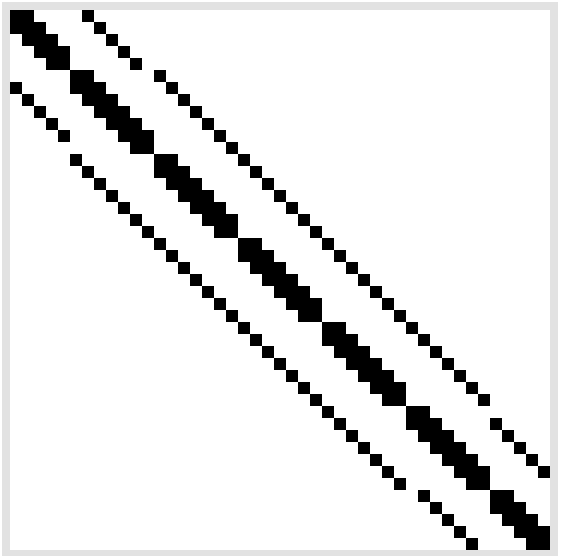
\includegraphics[width=0.26\linewidth]{figures/sparsity_pattern_no_text.png}
    \end{center}
    \caption{\scriptsize
        An example sparsity pattern for the finite element matrix of a 2D Poisson problem. White is zero and black is non-zero.
        The mesh has 61 vertices (16 on the boundary), and 104 triangles, resulting in a 45x45 system with 2025 entries, 197 non-zeros, and fill of $0.0973$.
    }
    \label{sparsity_pattern}
\end{figure}


Similar to the hat-functions-and-Voronoi-cells decomposition described for finite volumes,
the simplest scheme for the finite element Poisson equation is to triangulate $\Omega$ as
    $\bigcup_i T_i$
such that we have $n$ nodal points and $n_T$ triangles.
Each nodal point $p_i$ will be associated with a piecewise ``hat'' basis function $\phi_i$ which is $1$ at $p_i$ and
$0$ at its neighbours. Now, diverging from the previous finite volume method, the simplest thing we could do is let the trial functions be the same
as the test functions, $\psi_i = \phi_i$. This trivially gives a one-to-one correspondence between the $\phi_i$ and the $\psi_i$, which will lead
to a well-formed linear system.

\vskip 0.1in
(draw this)
\vskip 0.1in

% It is at this stage that, in a finite volume method, we would choose a test space and a cell decomposition in one-to-one correspondence
% with a basis of the test space.
% In that case,
% there was the obvious candidate of a polygonal cell per-vertex.
% However, there is a vast array of possible Galerkin ``decompositions'' of the domain.
% A ``finite element method'', in particular, uses test and trial basis functions of \textit{compact support}.

We have so far worked up to an instance of a \textit{finite element method}.
Finite element methods are characterised by a test space $\Phi$ and trial space
$\Psi$ with basis functions of \textit{compact support}, where $\Phi$ and $\Psi$ typically consist of continuous functions in
some Sobolev space, constructed over a domain tessellation.

\section{Implementing the finite element method for Poisson's equation}
We now have an effective algorithm for approximating the Poisson equation:
\begin{enumerate}
    \item Partition the 2D domain $\Omega$ into triangles $T_i$. This implicitly defines the hat basis functions $\phi_i = \psi_i$.
    \item Form the matrix and right-hand-side in \eqref{poisson_fem_matrix_equation}, by analytical or numerical integration.
    \item Solve the resulting linear system for $\hat{h}$, and construct the solution as $\Phi\cdot\hat{h}$.
\end{enumerate}
Each of these steps is conceptually well-separated into the domains of
mesh generation, matrix assembly, and numerical linear algebra.

\subsection{Mesh generation}
Mesh generation is itself a huge field. However, there are only two essentials for the handling of 2D meshes and piecewise-linear finite elements
--- a mesh data structure and a triangulator. Typically a mesh data structure will be provided by a separate library,
and the data organization (e.g., vertex, triangle, and adjacency information) will be designed to facilitate the kinds
of mesh traversals performed during matrix assembly. This is typically some variant of a ``halfedge'' data structure \cite{polygon_mesh_processing},
implemented in libraries such as Geometry Central \cite{geometry_central},
the Polygon Mesh Processing library \cite{polygon_mesh_processing_library}, and OpenMesh \cite{openmesh}.
A mesh data structure is a foundational component of \textit{mesh generation} systems. For 2D domains, a somewhat regular sampling of points on the boundary
and interior, followed by triangulation of these points, can suffice for a piecewise-linear finite element mesh.
The Triangle \cite{triangle} library, for example, contains a single very efficient and robust C routine (consisting of 16k lines of highly optimized code)
for performing Delaunay triangulations \cite{orourke}
on 2D domains,
with the specific goal of creating robust finite element meshes.


\subsection{Matrix assembly}
The matrix assembly stage is the core of a finite element implementation. The simplest idea is to iterate over all pairs $\phi_i$ and $\psi_j$,
letting $i=1,\cdots,n$, $j = 1,\cdots,n$, and approximate the integral $\int_\Omega \nabla\phi_i\cdot \nabla\cdot \psi_j\,dx$,
and store the value as entry $(i,j)$ of the matrix.
\begin{algorithm}
    \SetAlgoLined
    % \KwData{this text}
    % \KwResult{HOW}
    % initialization\;
    $M \leftarrow \text{zero matrix}$\;
    \For{$i=1,\cdots,n$}{
        \For{$j=1,\cdots,n$}{
            $M[i,j] \leftarrow \int_\Omega \nabla\phi_i\cdot \nabla\cdot \psi_j\,dx.$
        }
    }
\end{algorithm}

\begin{algorithm}
    % rhs computation
    \SetAlgoLined
    \For{$i=1,\cdots,n$}{
        $A \leftarrow 0$ \tcc*[l]{For computing total adjacent triangle areas.}
        \For{each triangle $T_j$ adjacent to $p_i$}{
            $A \leftarrow A + \text{Area}(T_j)$\;
        }
        $c \leftarrow g(p_i)$ \tcc*[l]{The source function is evaluated at the point $p_i$.}
        $\hat{b}[i] \leftarrow A\cdot c/3$\;
    }
\end{algorithm}

\begin{algorithm}
    % stiffness matrix computation and RHS boundary conditions.
    \SetAlgoLined

    $\text{Coefficients} \leftarrow \{\}$\;\tcc*[l]{This will contain triples $(i,j,\text{value})$ used to create the sparse matrix.}

    \For{each triangle $T_k$ in the domain partition}{
        $A \leftarrow \text{Area}(T_k)$\;
        $P,Q,R \coloneqq \text{The vertices of $T_k$}$\;
        $J \leftarrow \begin{bmatrix} Q_x-P_x & R_x-P_x \\ Q_y-P_y & R_y - P_y \end{bmatrix}$ \tcc*[l]{Jacobian of the reference transform.}
        $\text{Gradients} \leftarrow \left\{\begin{bmatrix} -1 & -1 \end{bmatrix},
                                            \begin{bmatrix} 1 & 0 \end{bmatrix},
                                            \begin{bmatrix} 0 & 1 \end{bmatrix}\right\}$\;
        $L \leftarrow \text{zero matrix}$ \tcc*[l]{The local stiffness matrix.}
        \For{$l,m=1,\cdots,3$}{
	    $L[l,m] \leftarrow A\left(\text{Gradients}[l] J^{-1}\right)\cdot\left(\text{Gradients}[m]J^{-1}\right)$\;
        }
        \For{$l,m=1,\cdots,3$}{
            \If{$p_{I(l)}$ is on the boundary}{skip\;}
            \If{$p_{I(m)}$ is on the boundary}{
                $\hat{b}[I(l)] \leftarrow \hat{b}[I(l)] - u_\Gamma(p_{I(m)})L(l, m)$\;
            }
            \Else{
                $\text{Coefficients} \leftarrow \text{Coefficients} \cup \left\{(I(l),I(m),L(l,m))\right\}$\;
            }
        }
    }
\end{algorithm}
    %     for (int i = 0; i < 3; i++) {
    %         for (int j = 0; j < 3; j++) {
    %             bool b1 = verts[i].on_boundary();
    %             bool b2 = verts[j].on_boundary();
    %             if (b1) {
    %                 continue; // The trial function can't be centered on the boundary.
    %             } else if (b2) {
    %                 auto p = geom.position[verts[j]];
    %                 double boundary_val = dirichlet_boundary_function(p.x(), p.z());
    %                 rhs[vertex_indices[verts[i]]] -= boundary_val*local_stiffness_matrix(i,j);
    %             } else {
    %                 coefficients.push_back(EigenTriplet(vertex_indices[verts[i]], vertex_indices[verts[j]], local_stiffness_matrix(i,j)));
    %             }
    %         }
    %     }

    % for (auto tri : geom.mesh.faces()) {
    %     Vertex verts[3];
    %     int vertex_index = 0;
    %     auto he = tri.halfedge();
    %     do {
    %         he = he.next();
    %         verts[vertex_index] = he.vertex();
    %     } while (++vertex_index < 3);

    %     auto A = geom.position[verts[0]];
    %     auto B = geom.position[verts[1]];
    %     auto C = geom.position[verts[2]];
    %     double triangle_area = 0.5*(B-A).cross(C-A).norm();

    %     // Compute the local stiffness matrix.
    %     Eigen::Matrix<double, 2,2> jacobian_matrix;
    %     jacobian_matrix <<
    %         B.x() - A.x(),  C.x() - A.x(),
    %         B.z() - A.z(),  C.z() - A.z();
    %     auto grad_transform = jacobian_matrix.inverse().transpose();
    %     Eigen::Matrix<double, 3,2> gradients;
    %     gradients <<
    %         -1,-1,
    %         1,0,
    %         0,1;
    %     Eigen::Matrix<double, 3,3> local_stiffness_matrix;
    %     for (int i = 0; i < 3; i++) {
    %         auto grad_i = grad_transform * gradients.row(i).transpose();
    %         for (int j = 0; j < 3; j++) {
    %             auto grad_j = grad_transform * gradients.row(j).transpose();
    %             local_stiffness_matrix(i,j) = triangle_area * grad_i.dot(grad_j); //*triangle_area ??????????????????????????????????????
    %         }
    %     }

    %     
    %     // Eigen::Matrix<double, 3,3> local_stiffness_matrix;
    %     // local_stiffness_matrix << 
    %     //     1, -0.5, -0.5,
    %     //     -0.5, 0.5, 0,
    %     //     -0.5, 0, 0.5;
    %     // local_stiffness_matrix *= 2*triangle_area;

    %     // i: Row, trial function.
    %     // j: Column, test function.

    %     for (int i = 0; i < 3; i++) {
    %         for (int j = 0; j < 3; j++) {
    %             bool b1 = verts[i].on_boundary();
    %             bool b2 = verts[j].on_boundary();
    %             if (b1) {
    %                 continue; // The trial function can't be centered on the boundary.
    %             } else if (b2) {
    %                 auto p = geom.position[verts[j]];
    %                 double boundary_val = dirichlet_boundary_function(p.x(), p.z());
    %                 rhs[vertex_indices[verts[i]]] -= boundary_val*local_stiffness_matrix(i,j);
    %             } else {
    %                 coefficients.push_back(EigenTriplet(vertex_indices[verts[i]], vertex_indices[verts[j]], local_stiffness_matrix(i,j)));
    %             }
    %         }
    %     }

    %     // std::cout << local_stiffness_matrix << "\n";
    %     // for (int i = 0; i < 3; i++) std::cout << (verts[i].on_boundary() ? "b " : "_ ");
    %     // std::cout << "\n";
    %     // std::cout << rhs << "\n";
    %     // getchar();
    % }

\subsection{Numerical linear algebra}
The solution of large linear systems is a vast topic in itself. Finite element solvers are typically clients
of standard, robust linear and non-linear solver libraries, such as Argonne National Laboratory's PETSc libraries \cite{petsc}
and the smaller-scale C\texttt{++} libraries Armadillo \cite{armadillo} and Eigen \cite{eigen}.
A finite element solver will typically pass either a full matrix to the linear solver (dense or sparse),
or provide the linear solver with callback routines that give the solver access to the system coefficients when they are needed.

\begin{figure}[H]
    \begin{center}
        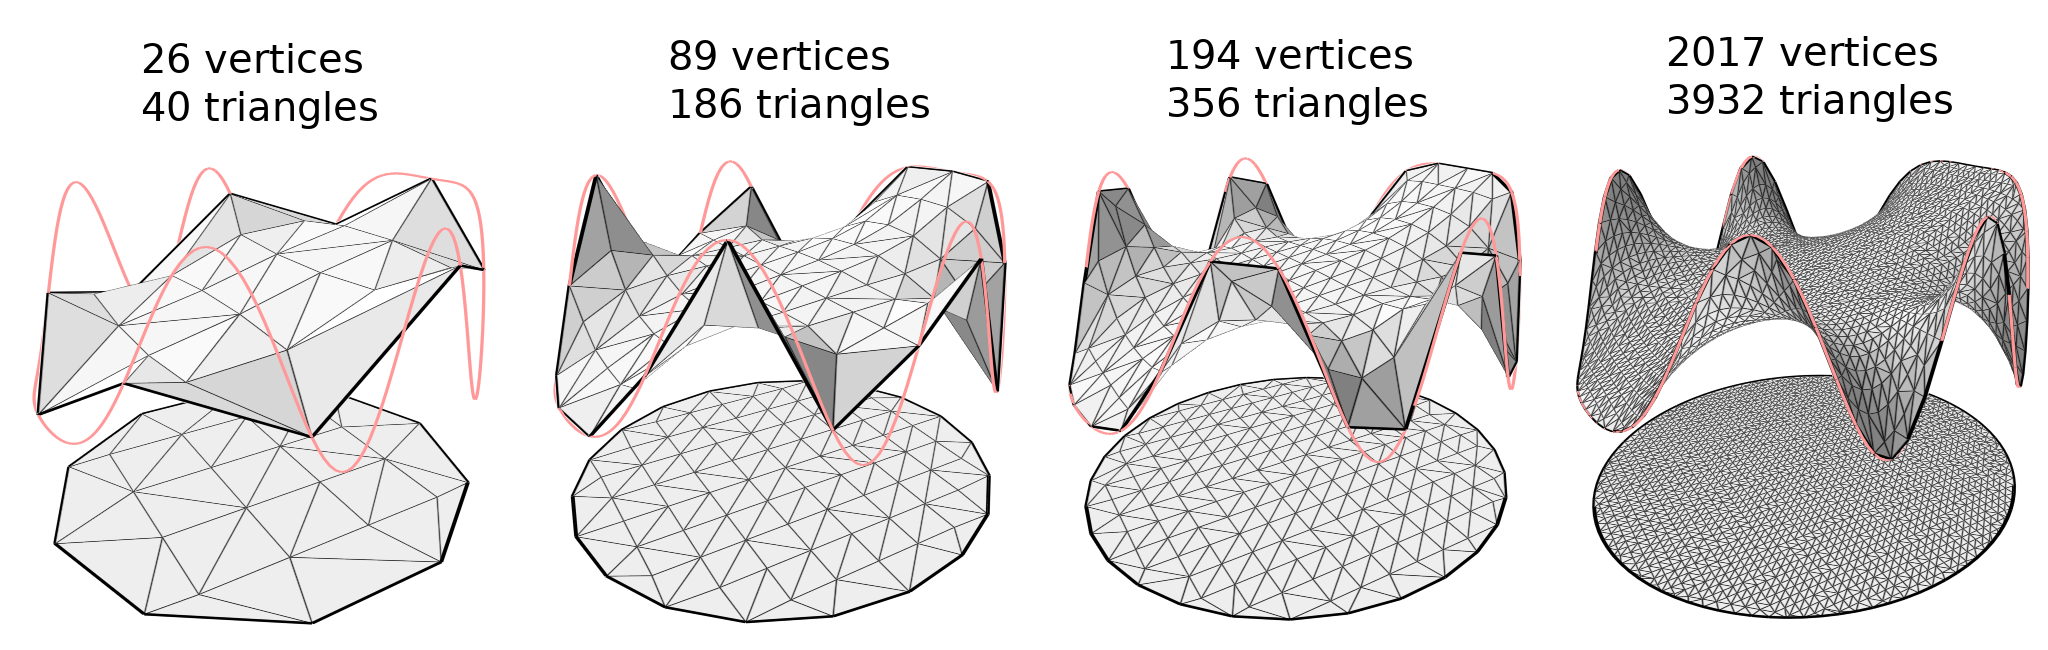
\includegraphics[width=\linewidth]{figures/laplace/laplacev2.png}
    \end{center}
    \caption{\scriptsize
        Text
    }
    \label{laplace_solution}
\end{figure}


% $$
%     h_\Gamma
% $$
% $$
%     \phi_\Gamma \in \Phi^*
% $$
% $$
%     \Gamma
% $$
% $$
%     T_1,\cdots,T_{n_T}
% $$


\chapter{Solving the Navier-Stokes equations}


\begin{thebibliography}{9}

\bibitem{newton}
Isaac Newton,
\textit{Philosophiae Naturalis Principia Mathematica (Third edition)},
1726.

\bibitem{johann_bernoulli}
Johann Bernoulli,
\textit{``Problema novum ad cujus solutionem Mathematici invitantur.'' (A new problem to whose solution mathematicians are invited.)},
1696.
(retrieved from wikipedia/brachistochrone\_curve)

\bibitem{dirichlet_principle}
A. F. Monna,
\textit{Dirichlet's principle: A mathematical comedy of errors and its influence on the development of analysis},
1975.

\bibitem{pde_larsson}
Stig Larsson,
\textit{Partial differential equations with numerical methods},
2003.

\bibitem{lax_1973}
Peter Lax,
\textit{Hyperbolic Systems of Conservation Laws and the Mathematical Theory of Shock Waves},
1973.

\bibitem{lanczos}
Cornelius Lanczos,
\textit{The Variational Principles of Mechanics},
1952.

\bibitem{batchelor}
G. K. Batchelor,
\textit{Introduction to Fluid Dynamics},
1967.

\bibitem{leal}
L. Gary Leal,
\textit{Advanced Transport Phenomena: Fluid Mechanics and Convective Transport Processes},
2007.

\bibitem{fem_ns}
Vivette Girault, Pierre-Arnaud Raviart,
\textit{Finite Element Methods for Navier-Stokes equations},
1986.

\bibitem{feynman_trick}
Richard Feynman,
\textit{Surely You're Joking, Mr. Feynman!},
1985.

\bibitem{arnold}
V.I. Arnol'd,
\textit{Mathematical Methods of Classical Mechanics},
1978.

\bibitem{turing}
Alan Turing,
\textit{The Chemical Basis of Morphogenesis},
1952.

\bibitem{applied_mathematics}
\textit{The Princeton Companion to Applied Mathematics},
2015.

\bibitem{polygon_mesh_processing}
Mario Botsch, Leif Kobbelt, Mark Pauly, Pierre Alliez, Bruno L\'evy,
\textit{Polygon Mesh Processing},
2010.

\bibitem{ddg_triangulated}
M. Meyer, M. Desbrun,  P. Schroder and A.H. Barr,
\textit{Discrete Differential-Geometry Operators for Triangulated 2-Manifolds},
2003.

\bibitem{ciarlet}
P. G. Ciarlet,
\textit{The Finite Element Method for Elliptic Problems},
1978.

\bibitem{tum}
Daniel Cremers,
\textit{Variational Methods in Computer Vision},
\\(https://vision.in.tum.de/teaching/online/cvvm)

\bibitem{evans}
Lawrence Evans,
\textit{Partial Differential Equations},
2010.

\bibitem{DOLFIN}
Documentation for DOLFIN-1.5.0 (Python),\\
(https://fenicsproject.org/olddocs/dolfin/1.5.0/python/index.html)

\bibitem{fenics_book}
Anders Logg, Kent-Andre Mardal, Garth N. Wells (editors),
\textit{The FEniCS book},
2012.

\bibitem{fenics_tutorial}
Hans Petter Langtangen, Anders Logg,
\textit{Solving PDEs in Python: The FEniCS tutorial I},
2016.

\bibitem{approximation_theory}
E. Ward Cheney,
\textit{Introduction to Approximation Theory},
1966.

\bibitem{stam}
Jos Stam,
\textit{Flows on surfaces of arbitrary topology},
2003.

\bibitem{ham_fem}
David Ham, Finite Element Course
(Imperial College London, 2013-2014),\\
http://wp.doc.ic.ac.uk/spo/finite-element/

\bibitem{fem_incompressible}
Howard Elman, David Silvester, Andy Wathen,
\textit{Finite Elements and Fast Iterative Solvers, with Applications in Incompressible Fluid Dynamics, 2nd edition},
2014.

\bibitem{strang_equilibrium}
Gilbert Strang,
\textit{A Framework for Equilibrium Equations},
1988.

\bibitem{brenner_scott}
Susanne C. Brenner, L. Ridgway Scott,
\textit{The Mathematical Theory of Finite Element Methods},
2008.

\bibitem{golub_van_loan}
Gene H. Golub, Charles F. Van Loan,
\textit{Matrix Computations, third edition},
1996.

\bibitem{triangle}
Jonathan Richard Shewchuk,
\textit{Triangle: Engineering a 2D Quality Mesh Generator and Delaunay Triangulator},
1996.

\bibitem{tetgen}
Hang Si,
\textit{TetGen: A quality tetrahedral mesh generator and a 3D Delaunay triangulator},
2015.

\bibitem{orourke}
Joseph O'Rourke,
\textit{Computational Geometry in C},
1998.

\bibitem{petsc}
Balay et al.,
PETSc web page, https://petsc.org/,
2021.

\bibitem{armadillo}
Conrad Sanderson, Ryan Curtin,
\textit{Armadillo: a template-based C++ library for linear algebra},
2016.

\bibitem{eigen}
Ga\"el Guennebaud,
\textit{Eigen: A C\texttt{++} linear algebra library},
2013.

\bibitem{geometry_central}
Nicholas Sharp, Keenan Crane, and others,
Geometry Central (surface mesh library), www.geometry-central.net,
2019.

\bibitem{polygon_mesh_processing_library}
Daniel Sieger, Mario Botsch,
The Polygon Mesh Processing Library,
http://www.pmp-library.org,
2020.

\bibitem{openmesh}
Leif Kobbelt,
OpenMesh (surface mesh library),
https://www.graphics.rwth-aachen.de/software/openmesh/,
2021.

\bibitem{one_hundred_years_galerkin}
Sergey Repin,
\textit{One hundred  years of the Galerkin method},
2017.

\bibitem{boris_galerkin}
Boris Galerkin,
\textit{Beams and plates. Series in some questions of elastic equilibrium of beams and plates (In Russian)},
1915.

\bibitem{sobolev_web_page}
Sobolev Institute of Mathematics,
Sergei Sobolev, biographical web page,
http://www.math.nsc.ru/conference/sobolev/english/About\_Sobolev\_SL.htm

\bibitem{firedrake}
Florian Rathgeber, David A. Ham, and others,
\textit{Firedrake: automating the finite element method by composing abstractions},
2016.


\end{thebibliography}
\end{document}
